\chapter{
    Potential Surface
    \\
    \large{Establishing What's Possible}
}
\label{sec:PotentialSurface}

As stated in the introduction, every person responds to lifting differently. This section is concerned with finding and establishing the limits of a given lifter within the context of a single exercise.

There are many limiting factors that need to be considered. How many reps can be done per set? How many sets can be done per exercise? What weight can the user lift given a particular amount of sets and reps? How much effort should the lifter exert to perform those sets and reps at the given weight? The answers to these questions form the thought process for the rest of the section.

When performing a single exercise, there are generally six things that dictate what is done:
\begin{enumerate}
    \item What exercise is being performed
    \item The number of sets being performed for a particular exercise
    \item The number of reps being performed for each set
    \item The weight each rep should be performed at
    \item The amount of effort expected to be exerted on each set
    \item The lifters current abilities
\end{enumerate}

The exercise being performed is largely dependent on what goals the lifter is pursuing as well as what weaknesses the lifter has. Due to the complexity of exercise selection as well as it's independence from the last five items on the list, it is explored in greater detail in a separate section. The last five items on that list have a large amount of dependence upon each other, and the relationship among them will be established in this section.

\section{Intuitive Relationships Between Variables}
\label{sec:PotentialSurfaceIntuitiveRelationshipsBetweenVariables}

A lifter has a \textit{volume tolerance}, which represents a lifters work capacity. Given a certain volume tolerance, the only five variables that can change are weight, intensity, effort, sets, and reps. This is obvious from equations \ref{eq:BaseVolumeEquation} and \ref{eq:IntensityBasedVolumeEquation}.

Weight and intensity are synonymous through the lens of volume, as the total amount of weight lifted is calculated regardless of the differing parameters. It should be clear from equations \ref{eq:BaseVolumeEquation} and \ref{eq:IntensityBasedVolumeEquation} that volume will increase with increased weight and intensity. Mathematically, this makes sense, but the limits of the human body need to be considered. As intensity approaches $100\%$ more effort is required to maintain the same amount of volume. Because effort is limited, volume will necessarily decrease at higher weights, to a point where it reverses the increase in volume from the increase in weight. An example may make this clearer. At $100\%$ intensity a lifter can realistically expect to obtain a volume equal to there 1RM, shown in equation \ref{eq:VolumeWithDiffereingIntensities1}. At $50\%$ intensity, all it takes is two reps to match the volume performed at $100\%$ intensity, which is shown in equation \ref{eq:VolumeWithDiffereingIntensities2}. At $50\%$ intensity, far more than one set of two reps can be performed, making it easy to surpass the volume done at $100\%$ intensity. The data in appendix \ref{sec:AppendixA} has many examples of this.

\begin{subequations}
    \begin{align}
        \label{eq:VolumeWithDiffereingIntensities1}
        v_{I=1}=&v(1,1,l_{1RM})=l_{1RM} \\
        \label{eq:VolumeWithDiffereingIntensities2}
        v_{I=0.5}=&v(1,2,0.5l_{1RM})=l_{1RM}
    \end{align}
\end{subequations}

It should be clear that volume will increase with weight until a peak is reached and from there will start to decrease because of limited effort at higher intensities. Where volume peaks exactly will need to be found from the data. Figure \ref{fig:IntensityVsVolumeGraph} is a graph comparing intensity and volume that clearly displays the intuitive behaviors discussed above.

\begin{figure}
    \centering
    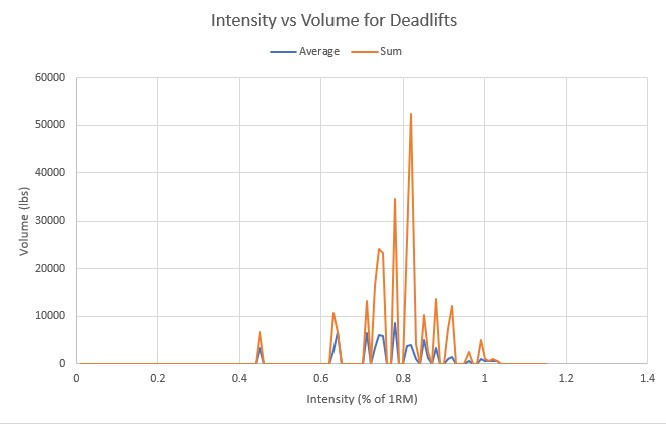
\includegraphics[scale=1.6]{graphs/IntensityVsVolumeGraph.jpg}
    \caption{A graph comparing intensity and volume. Note how there is a clear peak in volume near $80\%$.}
    \label{fig:IntensityVsVolumeGraph}
\end{figure}

With volume diminishing due to limited effort at higher intensities, the next question is what happens when effort increases or decreases across all intensities. As effort increases, more sets will be able to be completed, more reps will be able to be completed in each set, or more weight will be able to be lifted. If the increase in effort is large enough, some combination of sets, reps, and weight could all increase. The opposite is true if effort decreases. Again, from equations \ref{eq:BaseVolumeEquation} and \ref{eq:IntensityBasedVolumeEquation} it should be clear that sets and reps are directly proportional to volume, implying an increase in either one will increase volume. Putting all of this together, as effort increases volume will increase and as effort decreases volume will decrease.

\begin{figure}
    \centering
    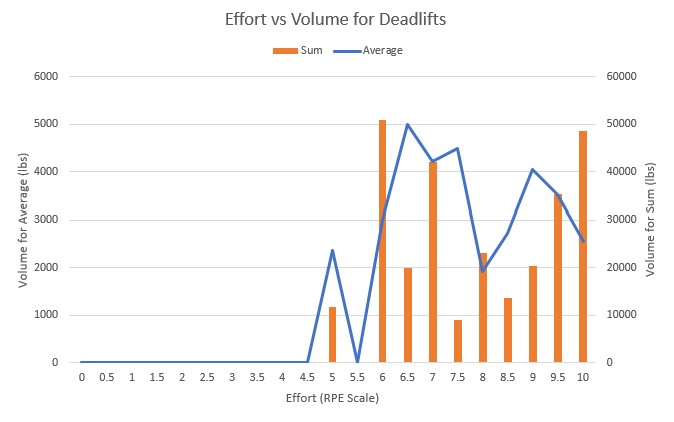
\includegraphics[scale=1.6]{graphs/EffortVsVolumeGraph.jpg}
    \caption{A graph comparing effort and volume. Note how volume tends to increase with higher effort values. The drop in volume at $E>7$ is likely from greater efforts generally having greater intensity, as shown in figure \ref{fig:EffortVsIntensity}.}
    \label{fig:EffortVsVolumeGraph}
\end{figure}
\begin{figure}
    \centering
    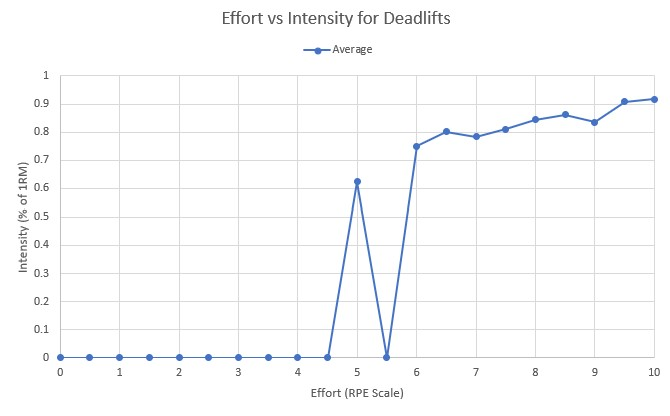
\includegraphics[scale=1.6]{graphs/EffortVsIntensityGraph.jpg}
    \caption{A graph comparing effort and average intensity. Note how the average intensity tends to increase with higher effort values. This is the result of a powerlifters goal being to maximize a 1RM. There are no data points in the range $0\le E\le 4.5$, making the average $0$.}
    \label{fig:EffortVsIntensity}
\end{figure}

In figure \ref{fig:EffortVsVolumeGraph} volume does seem to increase with effort, but after about $E=7$ it appears to decrease. This is a result of effort and intensity being correlated, which is shown in figure \ref{fig:EffortVsIntensity}. Effort and intensity being correlated is an artifact of the data being collected by a powerlifter, where the goal is to maximize the 1RM for a particular lift. As effort increases, a powerlifter will seek to maximize weight over volume. Combining the goal to maximize weight, and volume at higher intensities being necessarily limited by effort, the drop in volume after $E=7$ shown in figure \ref{fig:EffortVsVolumeGraph} is fully explained. Given a sport that is more concerned with rep maxes, such as crossfit, the effort vs intensity graph would level out because lower intensities would be pushed for as many reps as possible, creating a maximal effort set with a lower intensity. This would remove the drop in volume shown in the effort vs volume graph because higher effort sets would be performed with lower intensities that would allow the volume to continue to increase. This is also a perfect example to demonstrate how effort and intensity are two different concepts.

At this point, it may be tempting to conclude that volume should be constant given a particular weight and effort. This conclusion can be reached by looking at equations \ref{eq:BaseVolumeEquation} and \ref{eq:IntensityBasedVolumeEquation}, where once the weight and effort are known sets and reps would just vary inversely to ensure volume remains constant. Again, while mathematically true, the limits of the human body need to be considered. Evidence that the relationship between sets and reps is not inverse is shown in figure \ref{fig:SetsVsReps}, where a drop in reps from the expected inverse pattern is seen for $s<3$. This can be attributed to a lack of \textit{endurance}, where sets with a greater number of reps  require more endurance than sets with less reps. Powerlifters are eternally known for having no endurance, so it should come as no surprise that they will favor more sets over reps. This favoritism between sets and reps will of course mean volume is no longer constant given a particular weight and effort, and as such will be known as the \textit{volume skew}.

\begin{figure}[h]
    \centering
    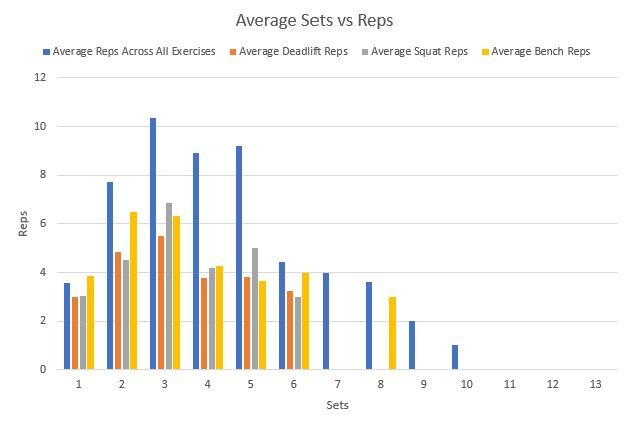
\includegraphics[scale=1.6]{graphs/SetsVsRepsGraph.jpg}
    \caption{A graph comparing average reps and sets. Note how the relationship is not perfectly inverse. In this case, the lifter has a volume skew towards sets, where more sets are favored (the long tail to the right), over reps (which would require a shorter tail and greater peak).}
    \label{fig:SetsVsReps}
\end{figure}

By this point it should be obvious the crux of the problem in question will require finding a lifters volume tolerance across weight and effort, as well as the lifters volume skew between sets and reps.

\section{Linear Regression and Time Series Problems}
\label{sec:PotentialSurfaceLinearRegressionAndTimeSeriesProblems}

With the goal to find a surface of best fit using the data set and linear regression, the limits of linear regression need to be considered. Looking at the data set, it should be clear that it is a time series: the data points are collected over time, and data points nearer in time have greater importance than data points farther away in time. Linear regression assumes that all the data points are uncorrelated, which was just proved to not be true. To reconcile the differences between working with linear regression and a time series data set, two things can be done.

The first step that can be taken is to limit the time frame that linear regression is run over. Sets, reps, volume, and the volume skew can all vary through time, but not necessarily in direct relation to time. As an example of this, consider seasonal training, which some powerlifters choose to employ. In the off season intensities will drop, volume will increase, and the emphasis on training may shift to hypertrophy over strength. In the on season intensities will increase, volume will necessarily decrease, and the emphasis on training will shift to strength over hypertrophy. This will result in shifts in the number of sets and reps being done over time. To capture these changes over time, the data points used will be limited to a specific time frame creating a form of a moving average as a lifter continues to train. Equation \ref{eq:TimeFrame} will be used to determine if a data point should be used while performing linear regression. The exact length of the time frame, $t_f$, will be discussed in section \ref{sec:TimeFrame}. Throughout the rest of this paper, equation \ref{eq:TimeFrame} will be written short hand as $t_i\in \{ T \}$.

\begin{equation}
    \label{eq:TimeFrame}
    \begin{split}
        %t_t\le t_i\le t_t+t_f
        t_i & \in\{ t_t, t_t+1,\dots,t_t+t_f \} \\
        \equiv t_i & \in \{ T \}
    \end{split}
\end{equation}
\centerline{where}
\begin{equation*}
    \begin{split}
        t_i &\equiv \text{The time component of an arbitrary data point }i \\
        t_t &\equiv \text{An arbitrary target time} \\
        t_f &\equiv \text{The time frame linear regression will be run over} \\
        T & \equiv \text{A shorthand notation representing the set of all allowed times}
    \end{split}
\end{equation*}

The second step that can be taken is to remove weights correlation with time. Weight correlating with time makes intuitive sense, as the goal of a powerlifter is to continually increase weight over time. As an example, say a lifter starts out with a 1RM of $300$ lbs on squat, but through training is able to increase that weight over time to $800$ lbs. It should be obvious from the example that weight has a positive correlation with time. To fix this, weight will be replaced by intensity. This will remove the correlation with time because intensity is calculated using an exercises 1RM, which itself changes with time, canceling out any effects from an increase in weight as time increases. Going back to the previous example, despite weight increasing over time, intensity would generally be limited to the range $0\le I\le 1$, because the lifter would set new 1RM's over time thereby forcing the intensities to be generally less than $1$.

By replacing weight with intensity, having an accurate tracking of a lifters 1RM over time becomes an important dependence for the model. For a powerlifter, this is generally not a problem as a lifts 1RM is usually tested once a mesocycle. Problems arise however when things like injuries, or other unplanned problems occur. During these situations a lifters 1RM is not known and can change rapidly or extremely slowly over time. A solution to problems like this will be explored in section \ref{sec:TimeFrameDynamicTimeFrameAnalysis} and \ref{sec:TimeFrameInjuriesAndChanges}.

\section{Defining the Relationships}
\label{sec:PotentialSurfaceDefiningTheRelationships}

To find a surface and run linear regression, the following subset of the data set is need.

\begin{equation}
    \label{eq:UserDataSet}
    \begin{split}
        \{(s,r,I,E)_i\}_{i=0}^n & \text{  where}\\
        \begin{split}
            s&\equiv \text{Sets} \\
            r&\equiv \text{Reps} \\
            I&\equiv \text{Intensity} \\
            E&\equiv \text{Effort} \\
        \end{split}
    \end{split}
\end{equation}

The inverse relationship between sets and reps mentioned in section \ref{sec:PotentialSurfaceIntuitiveRelationshipsBetweenVariables} leads to an initial representation of $sr=I$. This cannot be used however because of the asymptotic behavior of the equation at $x=0$ and $y=0$. It is not physically possible for a lifter to continually do infinitely more reps with infinitely less sets, or visa versa. This equation is also to rigid to account for any volume skew. The equation $s^2+r^2=I$ avoids asymptotic behavior and also allows for volume to be skewed, but can lead to a large peak in volume that cannot be controlled without reducing volume across the board. \footnote{This is the classical optimization problem presented in algebra classes, where the optimization equation is a parabola. In this case, the parabolic nature of the optimization equation, which represents some quasi-measure of volume, has to much 'volume' as the peak of the parabola is approached. A more level 'volume' equation is desired.} To avoid both problems, a combination of the equations will be used, which is shown below.

%The inverse relationship between sets and reps is mostly preserved, but the asymptotic behavior is also avoided.\footnote{The terms of the inverse relationship are both squared to make solving for $s$ and $r$ easier, which is something that will need to be done later.}

\begin{equation*}
    a(s-1)^2(r-1)^2+b(s-1)^2+c(r-1)^2=1-I
\end{equation*}

The above equation is negated so volume increases as intensity decreases and centered at $(s=1,r=1,I=1)$ to represent the users current 1RM. The constants $a$, $b$, and $c$ are left to be found by fitting the surface to the lifters data.

Effort also needs to be considered. The above equation could just be limited to fit a certain effort, or range of efforts, generating a set of equations, one for each effort or effort range. This sounds good initially, but the sparseness of the data set makes this approach prone to error. A given exercise may only be performed once per week, which gives very little data to work with in a four dimensional problem. Assuming perfect consistency, only 52 data points would be generated over a year. It is clear that every data point needs to be used if possible. Instead of only fitting the surface to data points that have a certain effort, the surface will be fit to all data points with an error proportional to the effort. Another constant, $d$, will be added so that the surface peaks at a weight that is appropriate for the target effort.

\begin{equation}
    \label{eq:PotentialSurfaceEquation}
    a(s-1)^2(r-1)^2+b(s-1)^2+c(r-1)^2+\epsilon E=d-I
\end{equation}
\centerline{where}
\begin{equation*}
    \begin{split}
        E & \in \{ 0,0.5,1,1.5,...,10 \} \\
        a,b,c,d & \ge 0 \\
    \end{split}
\end{equation*}

Equation \ref{eq:PotentialSurfaceEquation} is the final equation that fully realises all of the intuitive relationships discussed in section \ref{sec:PotentialSurfaceIntuitiveRelationshipsBetweenVariables}. This claim will be validated in sections \ref{sec:PotentialSurfaceVolumePeak} and \ref{sec:PotentialSurfaceVolumeIncreasesWithEffort}. Constraints have also been added to the constants in equation \ref{eq:PotentialSurfaceEquation} to limit the behavior of the model to what is sensible for the problem at hand. Keeping in mind the limitations discussed in section \ref{sec:PotentialSurfaceLinearRegressionAndTimeSeriesProblems}, linear regression can now be used to fit the surface to a lifters data, fully defining what that lifter is capable of doing.

The error equation is shown below.

\begin{equation*}
    E_{rr}=\sum_{
            \substack{i=0\\ t_i\in \{ T \}}
        }^n \left(
        I_i
        -d
        +a(s_i-1)^2(r_i-1)^2
        +b(s_i-1)^2
        +c(r_i-1)^2
        +\epsilon E
    \right)^2
\end{equation*}

The partial derivatives of each unknown constant are found, setting each equal to zero to minimize the error.

\begin{equation*}
    \begin{split}
        \frac{\partial E_{rr}}{\partial d}=
        \frac{\partial}{\partial d}\sum_{
                \substack{i=0\\ t_i\in \{ T \}}
            }^n \left(
            I_i
            -d
            +a(s_i-1)^2(r_i-1)^2
            +b(s_i-1)^2
            +c(r_i-1)^2
            +\epsilon E_i
        \right)^2&=0\\
        -2\sum_{
                \substack{i=0\\ t_i\in \{ T \}}
            }^n \left(
            I_i
            -d
            +a(s_i-1)^2(r_i-1)^2
            +b(s_i-1)^2
            +c(r_i-1)^2
            +\epsilon E_i
        \right)&=0\\
        d \sum_{\substack{i=0\\ t_i\in \{ T \}}}^n 1 
        -a \sum_{\substack{i=0\\ t_i\in \{ T \}}}^n (s_i-1)^2(r_i-1)^2
        -b \sum_{\substack{i=0\\ t_i\in \{ T \}}}^n (s_i-1)^2
        -c \sum_{\substack{i=0\\ t_i\in \{ T \}}}^n (r_i-1)^2
        -\epsilon \sum_{\substack{i=0\\ t_i\in \{ T \}}} E_i
        &=
        \sum_{\substack{i=0\\ t_i\in \{ T \}}}^n I_i\\
    \end{split}
\end{equation*}

After a similar process is carried out for each unknown constant, equation \ref{eq:LinearRegMatrixEquation} can be used, and the unknown constants can be solved for.

\begin{equation}
    \label{eq:LinearRegMatrixEquation}
    \left[
    \begin{matrix}
        \sum_{i=0}^n 1 &
        \dots &
        -\sum_{\substack{i=0\\ t_i\in \{ T \}}}^n E_i \\

        \sum_{\substack{i=0\\ t_i\in \{ T \}}}^n (s_i-1)^2(r_i-1)^2 &
        \dots &
        -\sum_{\substack{i=0\\ t_i\in \{ T \}}}^n E_i (s_i-1)^2(r_i-1)^2\\

        \vdots &
        \ddots &
        \vdots \\
        
        \sum_{\substack{i=0\\ t_i\in \{ T \}}}^n E_i &
        \dots &
        -\sum_{\substack{i=0\\ t_i\in \{ T \}}}^n E_i^2
    \end{matrix}
    \right]
    \left[
    \begin{matrix}
        d \\ a \\ \vdots \\ \epsilon
    \end{matrix}
    \right]=\left[
    \begin{matrix}
        \sum_{\substack{i=0\\ t_i\in \{ T \}}}^n I_i \\
        \sum_{\substack{i=0\\ t_i\in \{ T \}}}^n I_i(s_i-1)^2(r_i-1)^2 \\
        \vdots \\
        \sum_{\substack{i=0\\ t_i\in \{ T \}}}^n I_i E_i
    \end{matrix}
    \right]
\end{equation}

With equations \ref{eq:PotentialSurfaceEquation} and \ref{eq:LinearRegMatrixEquation} as well as the data set defined in equation \ref{eq:UserDataSet}, the surface that establishes what is possible for a lifter is fully defined. This surface will be called the \textit{potential surface}, and it is important to conceptualize that every combination of sets, reps, weight, and effort defined by this surface is theoretically possible for a lifter to complete. This is the base future sections of this paper will build off of.

After fitting the surface to the data shown in appendix \ref{sec:AppendixA} and discussed in section \ref{sec:DataSection}, graphs similar to the ones shown in table \ref{tab:DeadliftPotentialSurfaceAcrossEffort} were created. A full set of potential surface graphs for squat, bench, and deadlift across effort levels $5-10$ are available in appendix \ref{sec:AppendixB}. It is important the relationships discussed in section \ref{sec:PotentialSurfaceIntuitiveRelationshipsBetweenVariables} are present in these graphs, which will be the topic for sections \ref{sec:PotentialSurfaceVolumePeak}-\ref{sec:PotentialSurfaceUnboundedVolume}.

\begin{table}[]
    \centering
    \begin{tabular}{c|c}
        RPE & Potential Surface Graph \\
        \hline \\
        
        5 &
        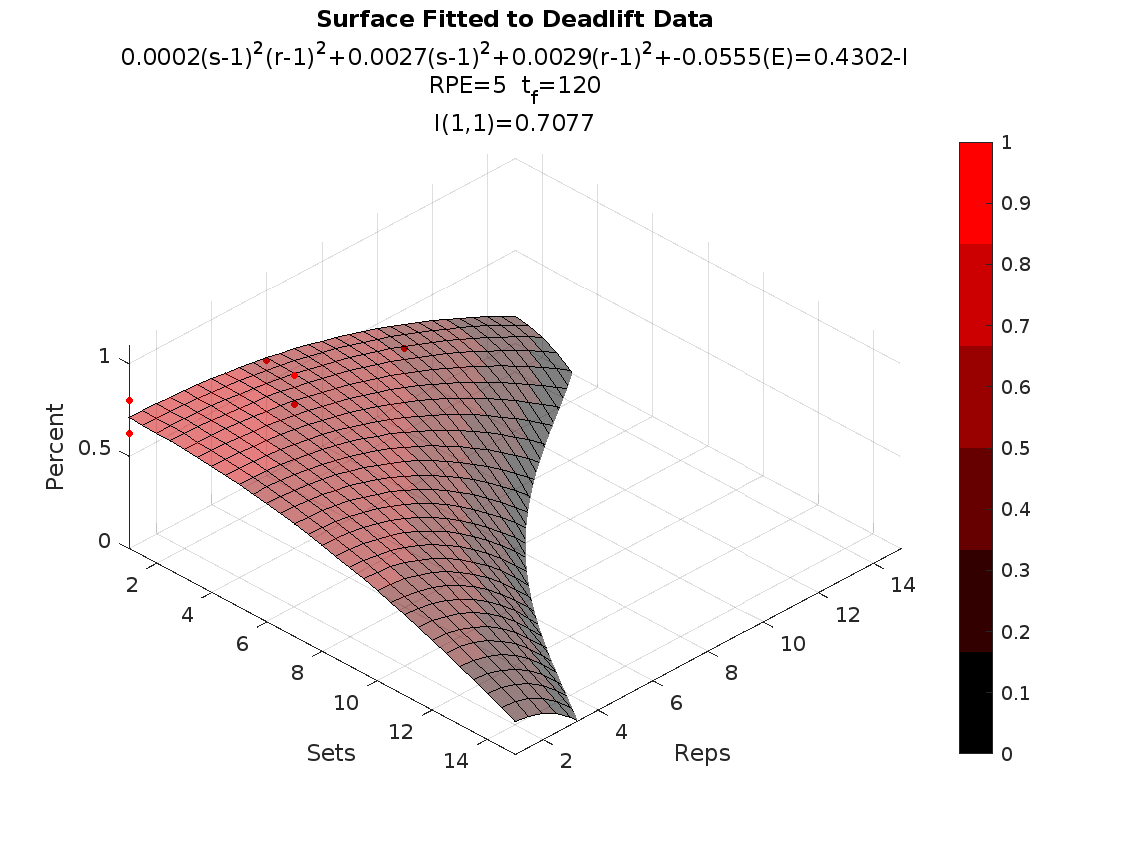
\includegraphics[width=139mm]{DeadliftSurface/5.png} \\
        10 &
        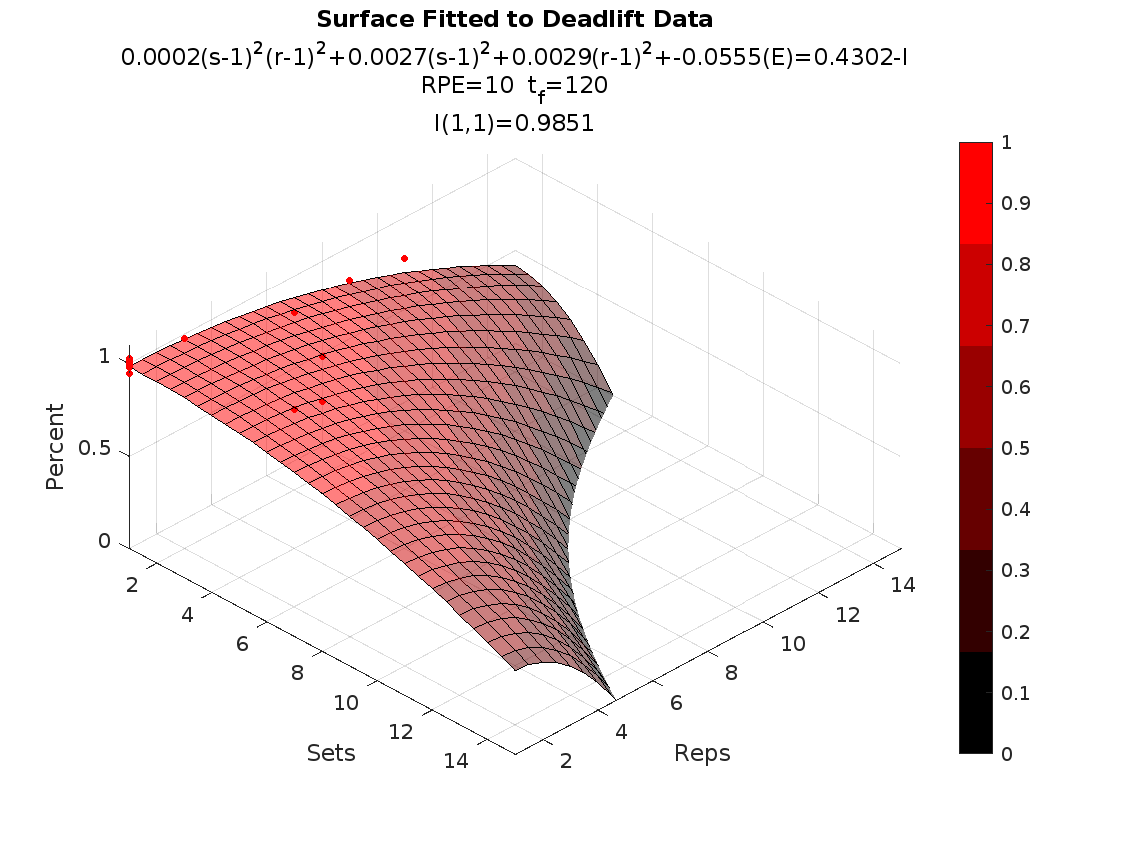
\includegraphics[width=139mm]{DeadliftSurface/10.png} \\
    \end{tabular}
    \caption{The potential surface fitted to deadlift data at various effort levels.}
    \label{tab:DeadliftPotentialSurfaceAcrossEffort}
\end{table}

Many of the relationships discussed in section \ref{sec:PotentialSurfaceIntuitiveRelationshipsBetweenVariables} are concerned with volume. To give some intuition for volume, the graphs shown in table \ref{tab:DeadliftVolumeAcrossEffort} are the result of solving the potential surface for $I$ and substituting it in equation \ref{eq:IntensityBasedVolumeEquation}.

\begin{table}[]
    \centering
    \begin{tabular}{c|c}
        RPE & Volume Graph \\%& Volume Across Intensities \\
        \hline \\
        
        5 &
        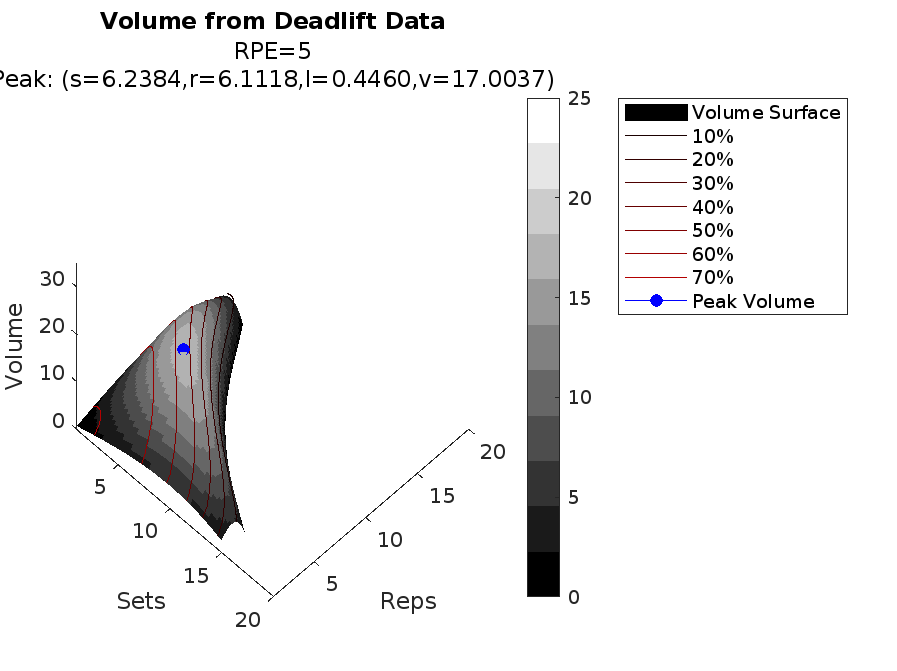
\includegraphics[width=139mm]{DeadliftVolume/5-1.png} \\%&  
        %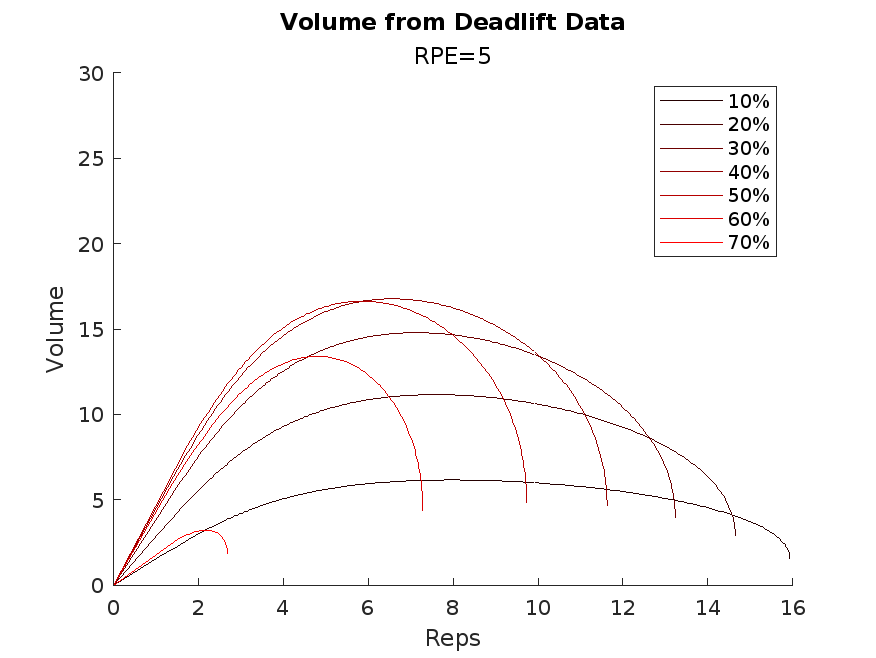
\includegraphics[width=76mm]{DeadliftVolume/5-2.png} \\
        
        %8 & 
        %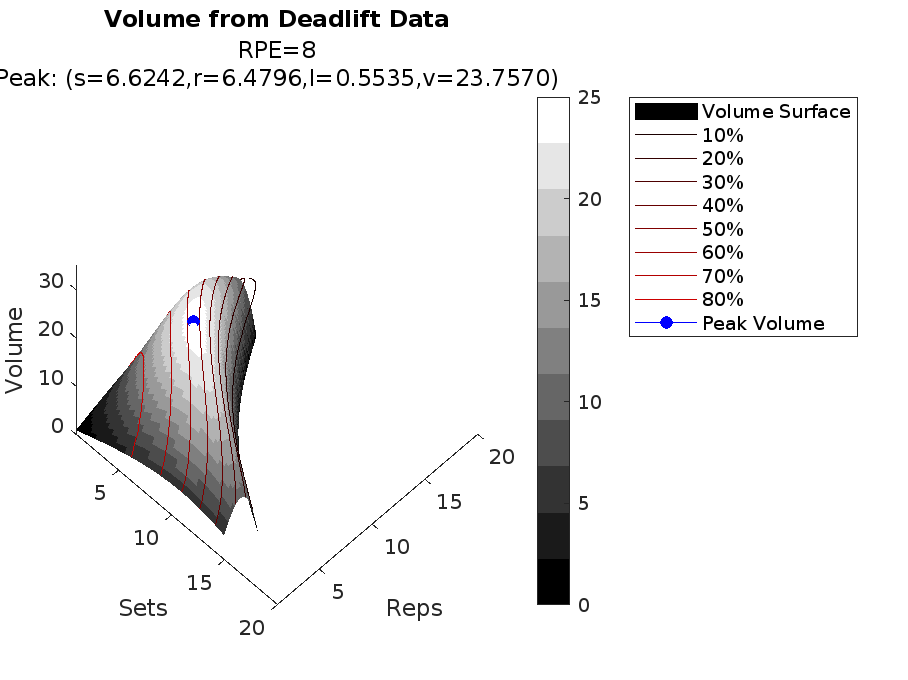
\includegraphics[width=90mm]{DeadliftVolume/8-1.png} \\%&
        %%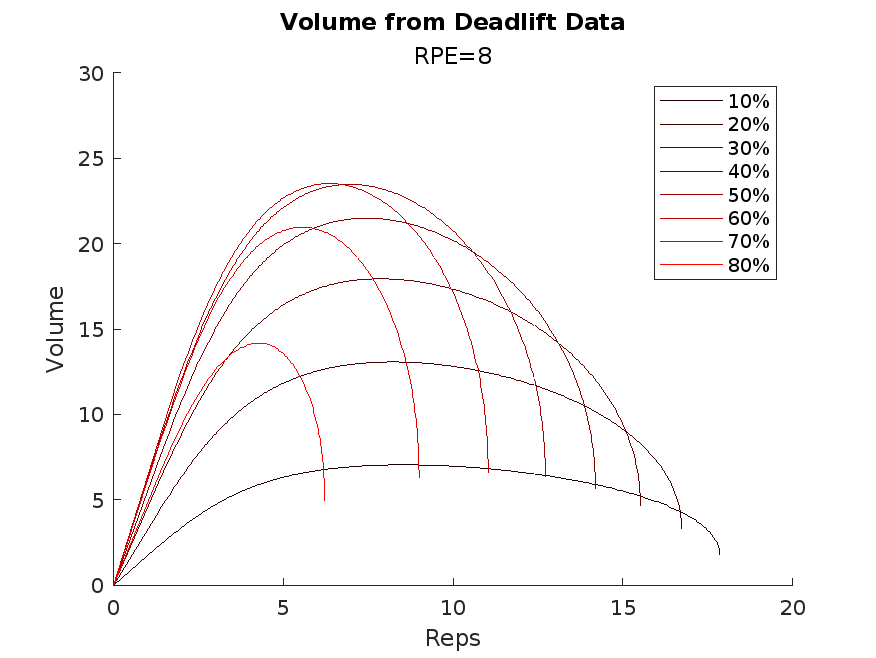
\includegraphics[width=76mm]{DeadliftVolume/8-2.png} \\
        
        10 &
        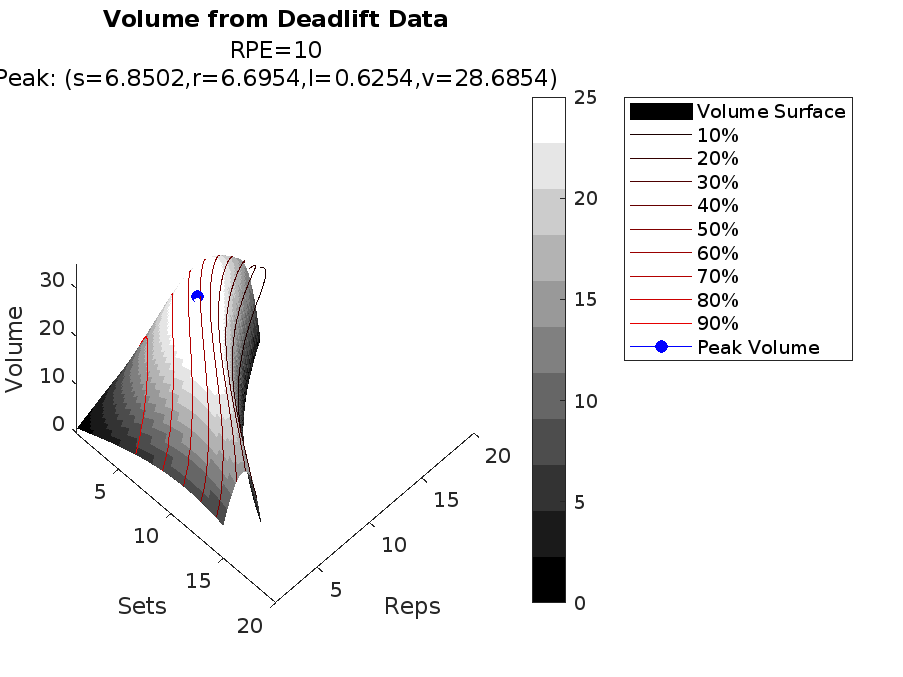
\includegraphics[width=139mm]{DeadliftVolume/10-1.png} \\%&
        %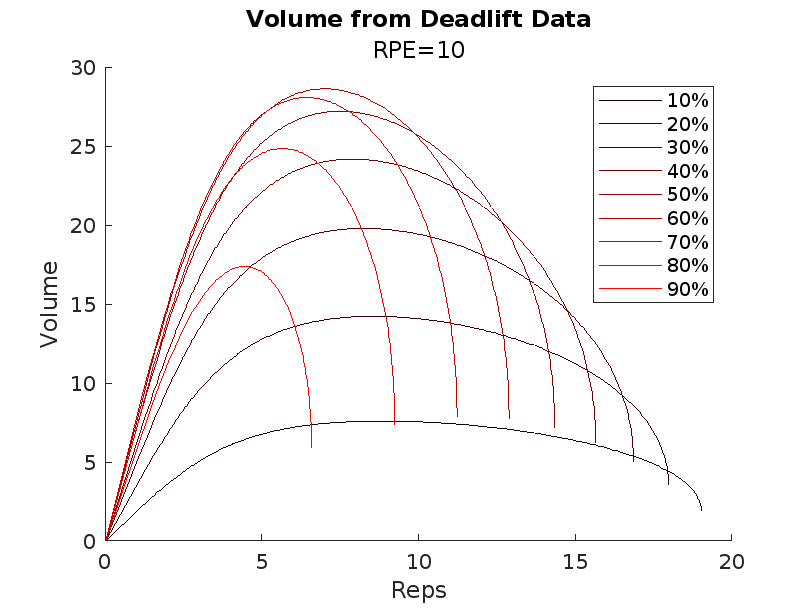
\includegraphics[width=76mm]{DeadliftVolume/10-2.png} \\
    \end{tabular}
    \caption{The volume equation from deadlift data at various effort levels. Volume was scaled linearly by $l_{1RM}$, making the vertical axis just $srI$. Note how there is a clear peak in volume as well as a ridge where volume rapidly decreases after crossing.}
    \label{tab:DeadliftVolumeAcrossEffort}
\end{table}


\section{Analysis: Proving Volume Increases With Weight Until a Peak Is Reached}
\label{sec:PotentialSurfaceVolumePeak}

It needs to be shown that, given a constant effort, volume increases with weight until a peak is reached at which point volume decreases. Analytically, this translates to finding the critical points and concavity of the volume equation. After solving equation \ref{eq:PotentialSurfaceEquation} for $s$ and substituting it in equation \ref{eq:IntensityBasedVolumeEquation}, equation \ref{eq:SetsSubedInVolume} is created and the process of finding critical points can be started. For simplicity, the volume equation will be scaled by $l_{1RM}$, removing its presence on the right hand side of the equation. The first and second partial derivatives of $v$ with respect to $I$ will also be needed.

\begin{equation}
    \label{eq:SetsSubedInVolume}
    v(r,I,E)=rI\left( \left( \frac{d-I-c(r-1)^2-\epsilon E}{a(r-1)^2+b} \right)^\frac{1}{2} +1 \right)
\end{equation}
\begin{equation}
    \label{eq:VolumeIPartialDerivative}
    \frac{\partial v}{\partial I} = 
    r+
    r\left( a(r-1)^2+b \right)^{-\frac{1}{2}} 
    \left( d-I-c(r-1)^2-\epsilon E \right)^\frac{1}{2}
    \left(
        1-\frac{I}{2}\left( d-I-c(r-1)^2-\epsilon E \right)^{-\frac{3}{2}}
    \right)
\end{equation}
\begin{equation}
    \label{eq:VolumeISecondPartialDerivative}
    \frac{\partial v'}{\partial I}=
    -r\left( a(r-1)^2+b \right)^{-\frac{1}{2}}
    \left( d-I-c(r-1)^2-\epsilon E \right)^{-\frac{1}{2}}
    \left(
        1+\frac{I}{4}\left( d-I-c(r-1)^2-\epsilon E \right)^{-1}
    \right)
\end{equation}

Both $\partial_Iv$ and $\partial_{II}v$ will need to be set to $0$ and solved for. When looking at $\partial_{II}v$, in order for a maximum to occur $\partial_{II}v<0$. Looking at the parenthetical groups of $\partial_{II}v$, the first two are guaranteed to be $\ge 0$.

\begin{enumerate}
    \item $r\ge0$ from section \ref{sec:UnitsOfMeasurement}
    \item $\left( a(r-1)^2+b \right)^{-\frac{1}{2}}>0$ from section \ref{sec:UnitsOfMeasurement} and the constraints placed on $a$ and $b$ in equation \ref{eq:PotentialSurfaceEquation}
\end{enumerate}

The third parenthetical group creates a further constraint for the current problem in question, and is shown in the inequality below. This constraint guarantees that the third parenthetical group is $>0$.

\begin{equation*}
    d-I-c(r-1)^2-\epsilon E>0
\end{equation*}

Given that the first three parenthetical groups are all $>0$, the last one must also be $>0$ in order for $\partial_{II}v$ to be $<0$. The inequality from the fourth parenthetical grouping is shown below. The constraint above nicely eliminates the imaginary part of the inequality.

\begin{equation*}
    I<\frac{4}{3}\left( d-c(r-1)^2-\epsilon E \right)
\end{equation*}

Before moving on, it is worth exploring what the above inequality has to say. As $r$ increases the range over which a maximum can occur in $I$ decreases. This may seem counter intuitive, but when considered from the perspective of volume it makes more sense. At the extreme, as the number of reps continue to increase volume continues to increase, which necessitates weight decreasing, making $I$ decrease. This is important because it shows the model respects the limitations that volume presents on weight.

Given the range where a maximum can occur, a critical point still needs to be found. This is not so easily done, and requires a computational approach. Using deadlift data, figure \ref{fig:DeadliftIntensityCriticalPoints} shows where the critical points are in relation to the region where a maximum can occur. It is clear that the critical points are all within the appropriate region to guarantee a maximum occurs.

\begin{figure}
    \centering
    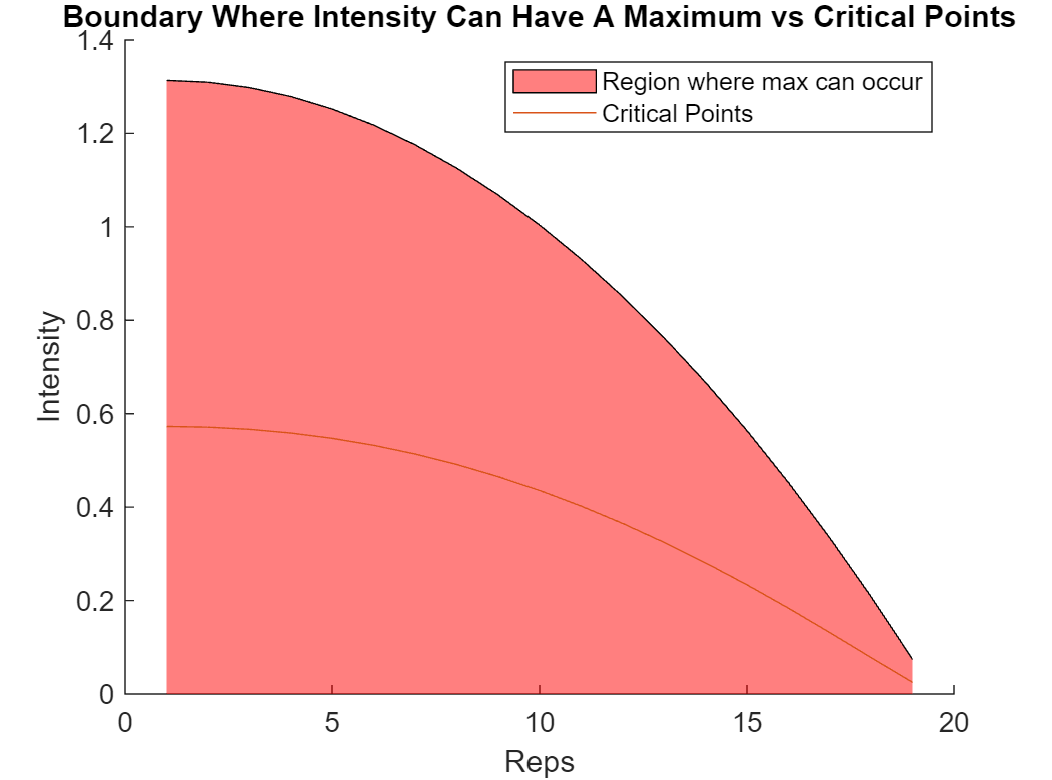
\includegraphics[width=140mm]{DeadliftConstants/IntensityCriticalPoints.png}
    \caption{Critical points for intensity from deadlift data and a time frame of 120 days with an effort of $E=5$. Note how they are all within the boundary where a maximum can occur.}
    \label{fig:DeadliftIntensityCriticalPoints}
\end{figure}

Before carrying on, it is worth mentioning that the same process used to find intensity critical points can be carried out but instead of solving equation \ref{eq:PotentialSurfaceEquation} for $s$, it can be solved for $r$. Doing this produces analogous analytical results, with $b$ and $c$ switching places along with $s$ and $r$. In order for the true peak in $I$ to be found, both approaches need to correspond to the same set of critical points. To help visualize any differences, the two sets of critical points can be plotted on top of the volume surface, as shown in figure \ref{fig:DeadliftIntensityCriticalPointsOnVolume}. From this figure, it should be clear that the two different ways to identify the peak in $I$ do not produce the same result.

\begin{figure}
    \centering
    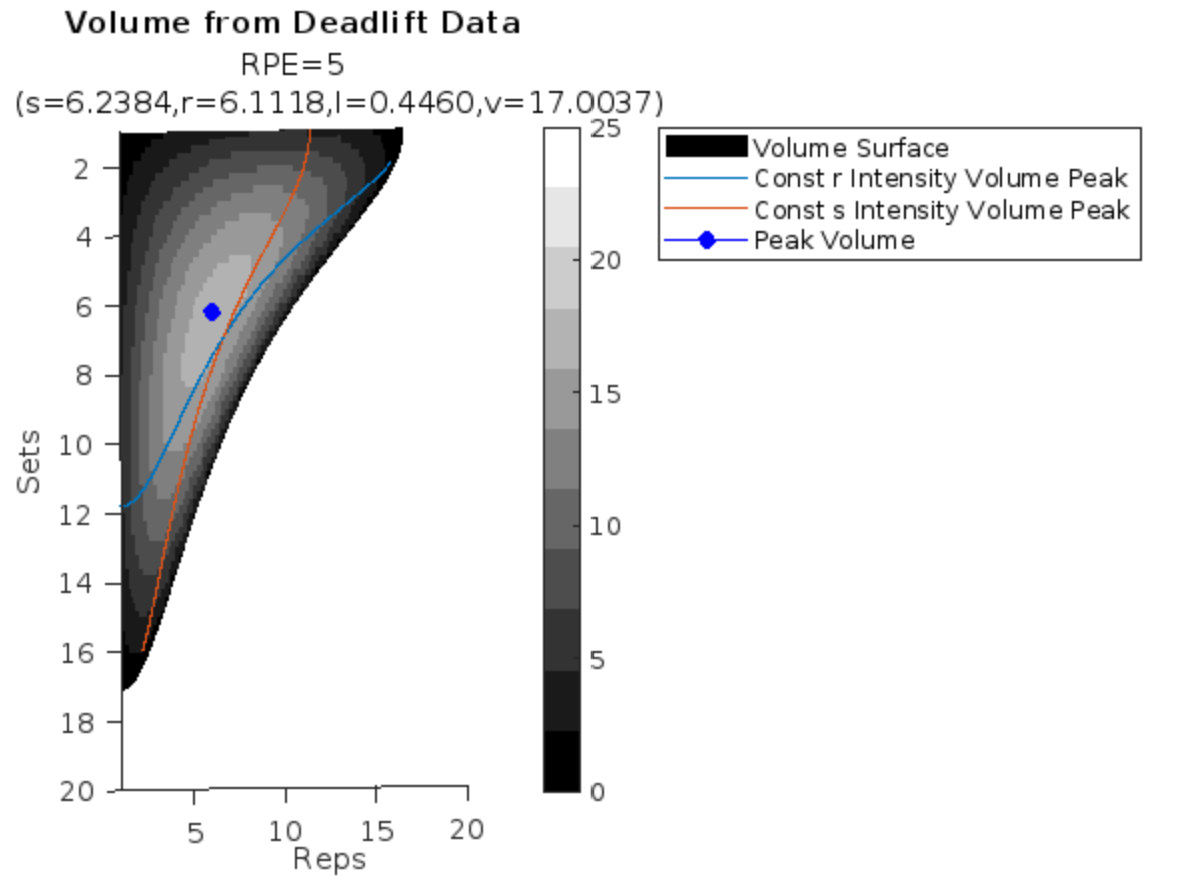
\includegraphics[width=140mm]{DeadliftConstants/IntensityCriticalPointsOnVolume.png}
    \caption{Intensity critical points graphed on the volume surface. These lines represent where intensity is maximized, in relation to constant $s$ and $r$ values.}
    \label{fig:DeadliftIntensityCriticalPointsOnVolume}
\end{figure}

The reason for the discrepancies in results can be explained by simplifying the problem to two dimensional approaches. The original three dimensional problem was reduced down to two different two dimensional problems, creating two separate ways to view the problem, and hence two different solutions. With an analytical approach failing to create consistent results, the graphs in table \ref{tab:DeadliftVolumeAcrossEffortOnlyIntensity} serve as the best proof that volume increases with effort until a peak is reached. These graphs do show some of the problems of viewing the problem from two dimensions. They show that volume does not always increase or decrease across intensity for all values of $r$. What does appear to increase across $I$ until a peak is reached is the peak volume.

\begin{table}
    \centering
    \begin{tabular}{c|c}
        RPE & Volume Across Intensities \\
        \hline
        
        5 &
        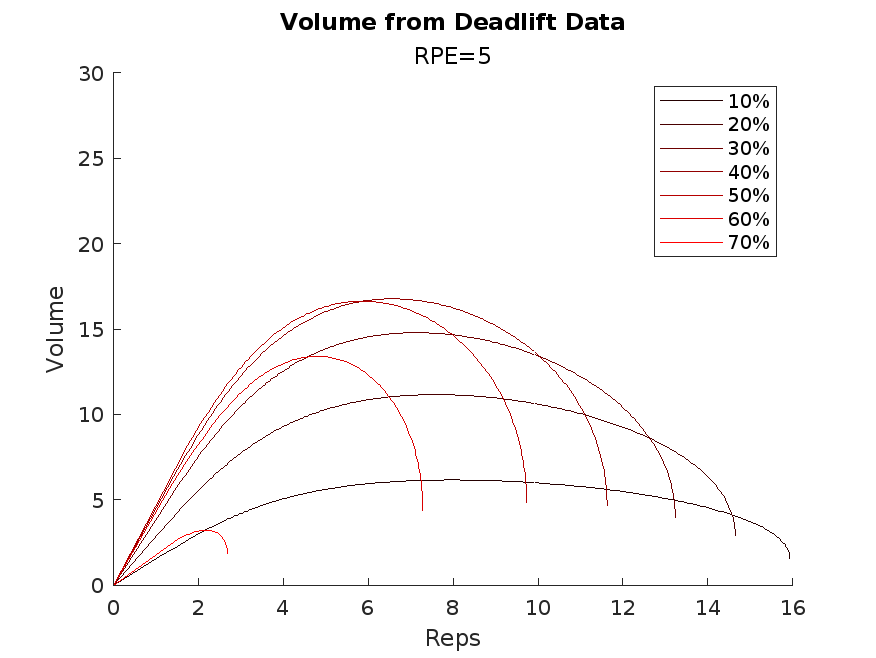
\includegraphics[width=140mm]{DeadliftVolume/5-2.png} \\
        
        %8 &
        %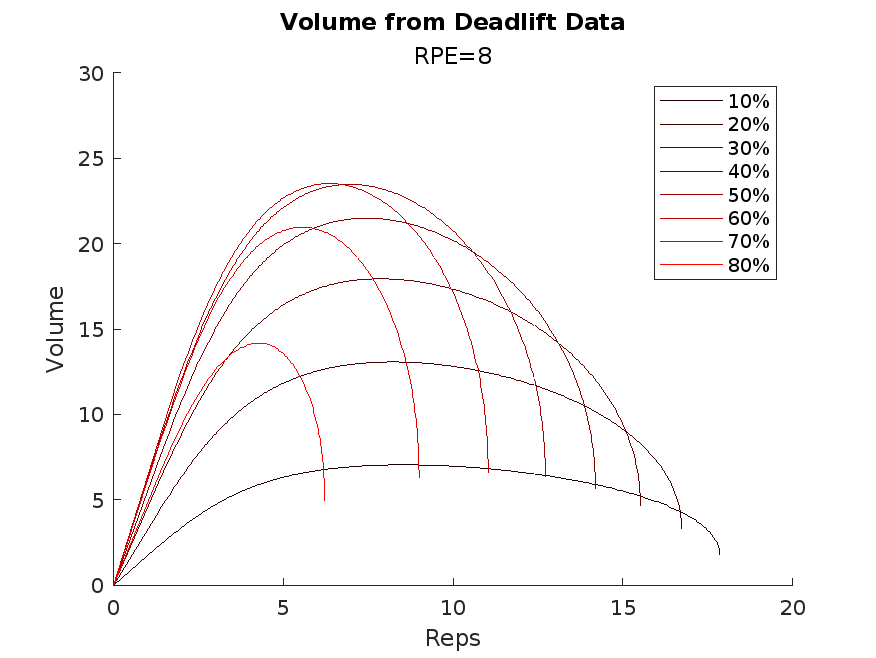
\includegraphics[width=76mm]{DeadliftVolume/8-2.png} \\
        
        10 &
        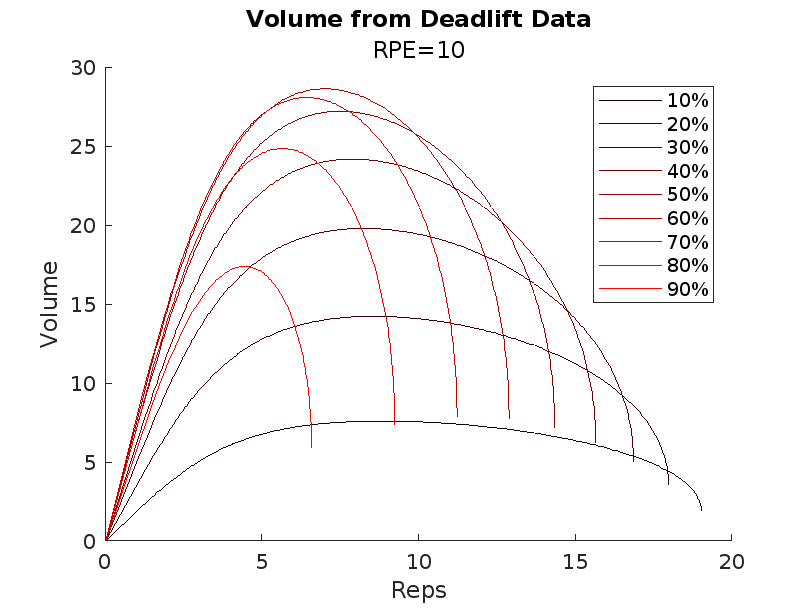
\includegraphics[width=140mm]{DeadliftVolume/10-2.png} \\
    \end{tabular}
    \caption{The same volume equation from table \ref{tab:DeadliftVolumeAcrossEffort} but only graphed across different intensities. Again, the vertical axis scaled by $l_{1RM}$. The intensity lines on the graphs in table \ref{tab:DeadliftVolumeAcrossEffort} correspond to the same intensity lines on these graphs.}
    \label{tab:DeadliftVolumeAcrossEffortOnlyIntensity}
\end{table}

%\begin{equation}
%    \label{eq:IntensitySubedInVolume}
%    v(s,r,E)=sr\left( d-a(s-1)^2(r-1)^2-b(s-1)^2-c(r-1)^2-\epsilon E \right)
%\end{equation}
%
%Finding each partial derivative of equation \ref{eq:IntensitySubedInVolume} is required. Effort is constant, making it unnecessary to find it's partial derivative.
%
%\begin{equation}
%    \label{eq:VolumeSPartialDerivative}
%    \begin{split}
%        \frac{\partial v}{\partial s}=&
%        \frac{\partial}{\partial s}sr\left( d-a(s-1)^2(r-1)^2-b(s-1)^2-c(r-1)^2 -\epsilon E \right) \\
%        =& rd-r\epsilon E-cr(r-1)^2-r\left( a(r-1)^2+b \right)\left( 3s^2-4s+1 \right)
%    \end{split}
%\end{equation}
%\begin{equation}
%    \label{eq:VolumeRPartialDerivative}
%    \begin{split}
%        \frac{\partial v}{\partial r}=&
%        \frac{\partial}{\partial r}sr\left( d-a(s-1)^2(r-1)^2-b(s-1)^2-c(r-1)^2 -\epsilon E \right) \\
%        =& sd-s\epsilon E-bs(s-1)^2-s\left( a(s-1)^2+c \right)\left( 3r^2-4r+1 \right)
%    \end{split}
%\end{equation}
%
%It should be obvious that setting equations \ref{eq:VolumeSPartialDerivative} and \ref{eq:VolumeRPartialDerivative} equal to $0$ and solving the system of equations for $s$ and $r$ is analytically impossible. As such, a computational approach is required. In the computational approach, graphing equation \ref{eq:IntensitySubedInVolume} will replace finding the concavity and gradient descent will replace solving the system of partial derivatives to get critical points. A couple graphs from equation \ref{eq:IntensitySubedInVolume} at varying effort levels are shown in table \ref{tab:DeadliftVolumeAcrossEffort}.


%Looking at the graphs in table \ref{tab:DeadliftVolumeAcrossEffort}, there is an obvious peak in volume. This peak however is not the peak in volume that needs to be identified. This peak represents the maximal possible volume across all valid intensities, sets, and reps given a constant effort. The peak in volume that needs to be identified is across all valid sets and reps given a constant intensity and effort. Despite this, for the purpose of establishing landmark values, this peak will be solved for, which will require gradient descent as shown in equation \ref{eq:VolumePeakGradientDescent}. The graphs in table \ref{tab:DeadliftVolumeAcrossEffort} identify the peak volume.
%
%\begin{equation}
%    \label{eq:VolumePeakGradientDescent}
%    \vec{v}_{n+1}=\vec{v}_{n}+\mu\nabla v_{s}(\vec{v}_{n})=\vec{v}_{n}+\mu
%    \left[
%        \begin{matrix}
%            \frac{\partial v}{\partial s}(\vec{v}_{n}) \\
%            \frac{\partial v}{\partial r}(\vec{v}_{n})
%        \end{matrix}
%    \right]
%\end{equation}
%
%Besides having a peak, there is also a ridge where once crossed volume drops drastically. This ridge is the peak in volume that needs to be verified. In order for volume to increase with weight until a peak is reached, this ridge and any lines parallel to it on the volume surface need to each have a constant intensity. It appears that the intensity lines on the graphs in table \ref{tab:DeadliftVolumeAcrossEffort} are parallel to the ridge. If only the intensity lines are graphed, as shown in table \ref{tab:DeadliftVolumeAcrossEffortOnlyIntensity}, volume seems to reach a peak across intensities. Given this, there is reason for further investigation.
%
%\begin{table}[]
%    \centering
%    \begin{tabular}{c|c}
%        RPE & Volume Across Intensities \\
%        \hline \\
%        
%        5 &
%        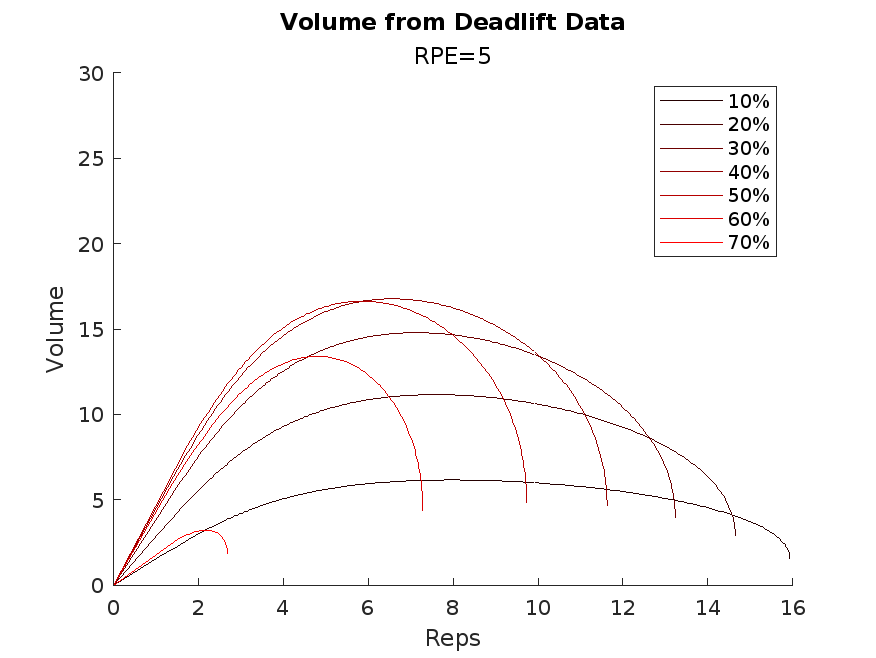
\includegraphics[width=140mm]{DeadliftVolume/5-2.png} \\
%        
%        %8 &
%        %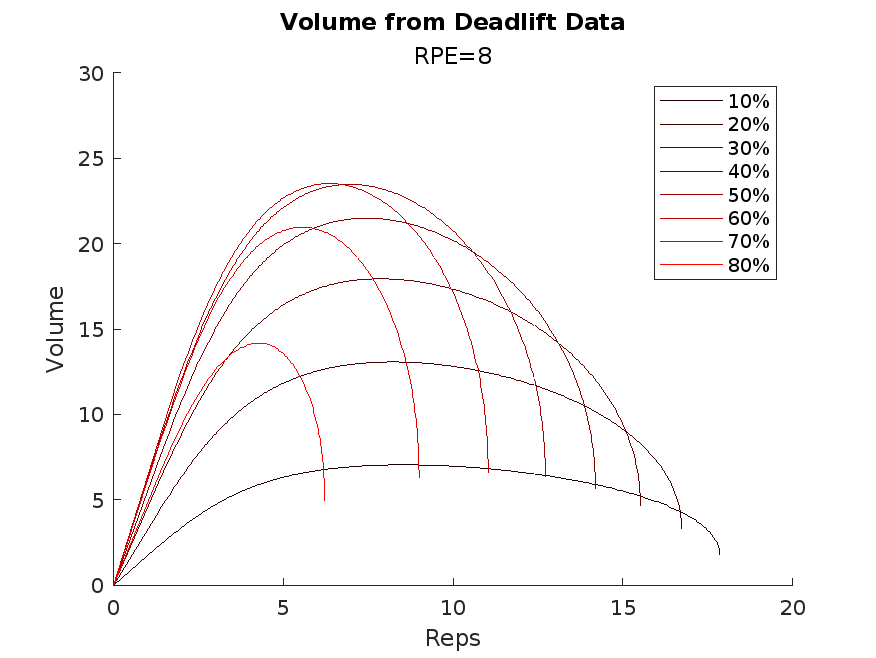
\includegraphics[width=76mm]{DeadliftVolume/8-2.png} \\
%        
%        10 &
%        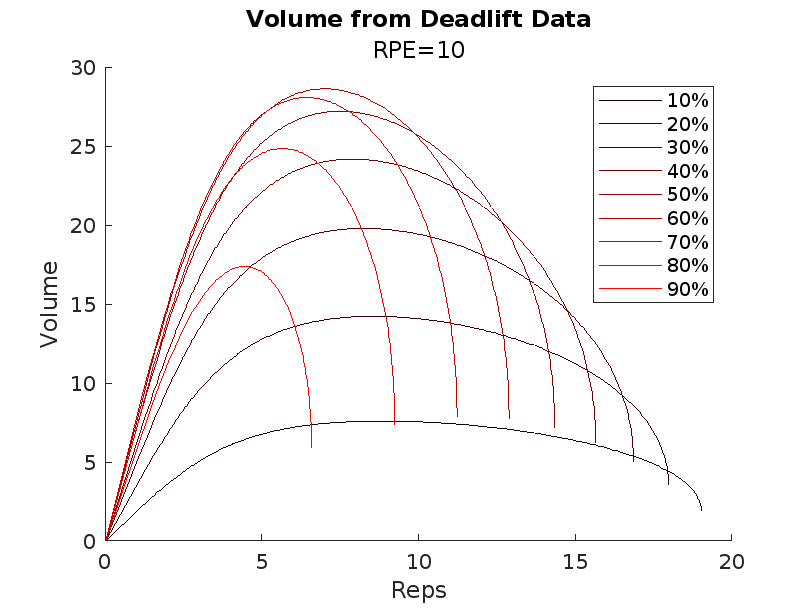
\includegraphics[width=140mm]{DeadliftVolume/10-2.png} \\
%    \end{tabular}
%    \caption{The same volume equation from table \ref{tab:DeadliftVolumeAcrossEffort} but only graphed across different intensities. The intensity lines on the graphs in table \ref{tab:DeadliftVolumeAcrossEffort} correspond to the same intensity lines on these graphs. Traveling from left to right on these graphs correspond to a clockwise rotation on the graphs in table \ref{tab:DeadliftVolumeAcrossEffort}.}
%    \label{tab:DeadliftVolumeAcrossEffortOnlyIntensity}
%\end{table}
%
%Proving the ridge and any lines parallel to it on the volume surface are all be the same intensity will be a two step process. First, the intensity values along the ridge will need to be identified to show they are constant. Once that is shown, intensities on lines parallel to the ridge will be identified to show they are constant.

%To identify the ridge one variable will be held constant and the opposite variables partial derivative will be set equal to zero and solved for. By doing this, the surface is essentially split up in an infinite set of lines, where each line is valid for a specific value of the constant variable. The peak of each line can then be identified. When all the lines peaks are stitched back together, they will all coalesce to create a new line that identifies the ridge. 

%Identifying the ridge is somewhat difficult. The first attempt held one variable constant and set the opposite variables partial derivative to $0$. Equation \ref{eq:VolumeRidgeConstS} is the result of setting the partial derivative of $v$ with respect to $r$ equal to $0$ and holding $s$ constant. Equation \ref{eq:VolumeRidgeConstR} does the same except $r$ is held constant. The idea was that the surface would essentially be sliced up in an infinite set of lines, where each line is valid for a specific value of the constant variable. The peak of each line can then be identified. When all the lines peaks are stitched back together, they will all coalesce to create a new line that identifies the ridge.
%
%\begin{subequations}
%    \begin{align}
%        \label{eq:VolumeRidgeConstS}
%        3r^2-4r+\left( 1-\frac{d-b(s-1)^2-\epsilon E}{a(s-1)^2+c} \right)&=0 \\
%        \label{eq:VolumeRidgeConstR}
%        3s^2-4s+\left( 1-\frac{d-c(r-1)^2-\epsilon E}{a(r-1)^2+b} \right)&=0
%    \end{align}
%\end{subequations}
%
%Doing this however forced a three dimensional problem into a two dimensional one, which created inconsistent results, as shown in figure \ref{fig:VolumeRidgeIdentFail}. Part of the problem is how mathematically vague the term 'ridge' is. As the work above shows, depending on how the surface is looked at 'ridge' will take different meanings.
%
%\begin{figure}
%    \centering
%    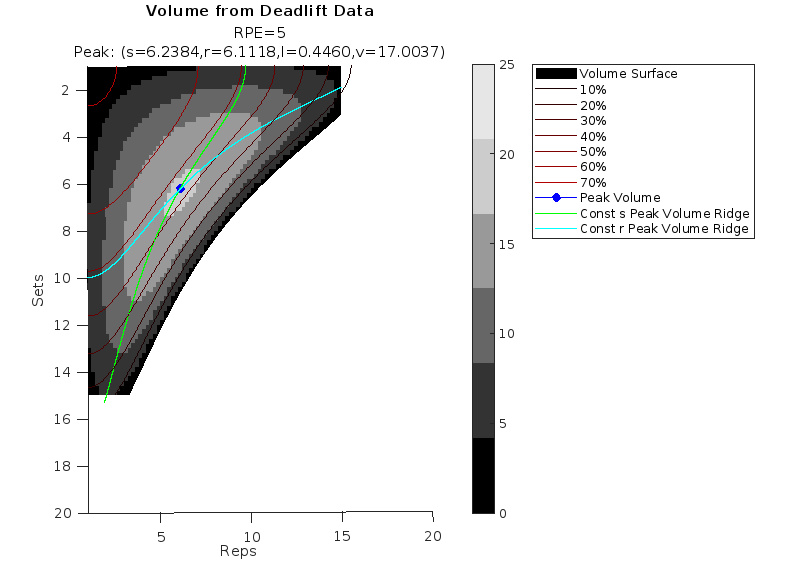
\includegraphics[width=170mm]{DeadliftVolume/FailedRidgeIdentification-2.png}
%    \caption{The first attempt at identifying the ridge. Note how the green and blue lines are not consistent with each other.}
%    \label{fig:VolumeRidgeIdentFail}
%\end{figure}
%
%While the results shown in figure \ref{fig:VolumeRidgeIdentFail} are far from perfect, some intuition can still be gained. The $50\%$ intensity line is very consistent with the two halves of the constant $s$ and constant $r$ ridge lines. This leads to the presumption that if the surface were split up into radial lines and the same process followed, a line very similar to the $50\%$ intensity line would result. While there is some basis in this approach, as equation \ref{eq:PotentialSurfaceEquation} is partially defined as an elliptic paraboloid which is circular in nature, more reasoning would be required to follow this approach.

%The second attempt to identify the ridge took a slightly different route. It started with a different volume equation, where instead of substituting equation \ref{eq:PotentialSurfaceIntensityEquation} in $v$, it substituted \ref{eq:PotentialSurfaceSetsEquation} in $v$. This allowed for the partial derivative with respect to $I$ to be taken, creating a far more direct approach than the previous attempt.

%Potentially discuss how lower intensities have more constant volume

\section{Analysis: Proving Intensity and Volume Increases With Effort}
\label{sec:PotentialSurfaceVolumeIncreasesWithEffort}

It needs to be shown that volume increases with increased effort and decreases with decreased effort. As such, the changes in $v$ relating to changes in $E$ are desired, requiring the partial derivative of equation \ref{eq:IntensitySubedInVolume} with respect to $E$.

\begin{equation}
    \label{eq:VolumeEPartialDerivative}
    \frac{\partial v}{\partial E}=
    \frac{\partial}{\partial E}srl_{1RM}\left( d-a(s-1)^2(r-1)^2-b(s-1)^2-c(r-1)^2-\epsilon E \right)=-srl_{1RM}\epsilon
\end{equation}

If $\partial_{E}v$ is always $>0$, then it can be said the function is strictly increasing, meaning volume strictly increases with increased effort. The following inequalities are given in section \ref{sec:UnitsOfMeasurement}.

\begin{equation*}
    \begin{split}
        s \ge & 1 \\
        r \in & \{ \mathbb{R}\ge 1 \} \\
        w > & 0 \\
    \end{split}
\end{equation*}

Given that $l_{1RM}$ is a weight, the following conclusion can be made given the above inequalities.

\begin{equation*}
    -srl_{1RM}\epsilon> 0 \textbf{ iff } \epsilon< 0
\end{equation*}

Therefore, it can be concluded that volume increases with increased effort \textbf{iff} $\epsilon< 0$. A similar argument can be made that proves volume decreases with decreased effort \textbf{iff} $\epsilon< 0$. If $\partial_E I$ is taken instead of $\partial_E v$, an analogous proof could be made to show that intensity increases with effort \textbf{iff} $\epsilon<0$.

Having the restriction that $\epsilon\le 0$ may seem problematic, but the $\epsilon$ value shown in table \ref{tab:DeadliftPotentialSurfaceAcrossEffort} is negative. For added reassurance, the $\epsilon$ values for three different exercises are all shown in table \ref{tab:EpsilonAcrossExercies}, and are all negative. It is clear the model is correctly identifying patterns from the training data and making volume increase with effort.

\begin{table}[h]
    \centering
    \begin{tabular}{c|c}
        Exercise & $\epsilon$ \\
        \hline
        Squat & -0.0461\\
        Bench & -0.0363\\
        Deadlift & -0.0555\\
    \end{tabular}
    \caption{The $\epsilon$ values for three different exercises. They are all negative, meaning the model is correctly making volume increase with effort.}
    \label{tab:EpsilonAcrossExercies}
\end{table}

\section{Analysis and Application: Volume Skew and Abstractly Describing Training}
\label{sec:PotentialSurfaceAbstractlyDescribingTraining}

The last intuitive relationship discussed in section \ref{sec:PotentialSurfaceIntuitiveRelationshipsBetweenVariables} is volume skew. As such, it needs to be shown that the model is capable of determining volume skew. Looking at figure \ref{fig:DeadliftIntensityCriticalPointsOnVolume} there is a clear skew towards sets with the surface reaching greater values on the set axis than the rep axis. This is consistent with the data presented in figure \ref{fig:SetsVsReps}, and is all that is needed to prove that the model can correctly identify volume skew.

Given the model can determine a volume skew, a way to represent it would be convenient. The meaning of the constants that were presented in the linear regression should be considered. The relative magnitude of constants $b$, and $c$ control how much volume can be completed favoring sets or reps respectively. As such, the ratio of $b$ to $c$, shown in equation \ref{eq:VolumeSkew}, presents itself as a way to measure volume skew. By measuring volume skew using the constants from linear regression, it is averaged across all weights and effort levels.

\begin{equation}
    \label{eq:VolumeSkew}
    v_s(b,c)=\frac{b}{c}
\end{equation}

Before continuing, the effects on equation \ref{eq:PotentialSurfaceEquation} from changes to $b$ and $c$ need to be considered. As such, equation \ref{eq:PotentialSurfaceEquation} is solved for $I$ and the partial derivative with respect to $b$ is taken. 

\begin{equation}
    \label{eq:VolumeBPartialDerivative}
    \frac{\partial I}{\partial b}=
            \frac{\partial}{\partial b} \left( d-a(s-1)^2(r-1)^2-b(s-1)^2-c(r-1)^2-\epsilon E \right)
\end{equation}

If $\partial_{b}I$ is always $\le 0$, then it can be said the function is strictly decreasing.

\begin{equation*}
    \frac{\partial}{\partial b} \left( d-a(s-1)^2(r-1)^2-b(s-1)^2-c(r-1)^2-\epsilon E \right) \le 0
\end{equation*}
\begin{equation*}
    (s-1)^2 \ge 0
\end{equation*}
\begin{equation*}
    s \ge 1
\end{equation*}

From section \ref{sec:UnitsOfMeasurement} it is guaranteed that $s\ge 1$, meaning that $I$ increases with decreases in $b$. A similar argument can be made that proves $I$ increases with decreases in $c$.

Keeping in mind how changes to $b$ and $c$ effect equation \ref{eq:PotentialSurfaceEquation}, a few initial observations can be made about equation \ref{eq:VolumeSkew}.

\begin{enumerate}
    \item If $v_s<1$ then $b<c$, which implies that the lifter favors sets for the given exercise, or has a volume skew towards sets for the given exercise.
    \item If $v_s>1$ then $b>c$, which implies that the lifter favors reps for the given exercise, or has a volume skew towards reps for the given exercise.
    \item If $v_s=1$, then the lifter has no volume skew.
    \item If $b=0$ or $c=0$ then a lifter has the maximum possible skew towards sets or reps respectively. \footnote{This idea will be explored more from volumes perspective in section \ref{sec:PotentialSurfaceUnboundedVolume}.}
\end{enumerate}

Table \ref{tab:VolumeSkewAcrossExercises} shows the constants and volume skew for three different exercises. As anticipated from the data in figure \ref{fig:SetsVsReps}, the volume skew favors sets over reps for all three exercises.

\begin{table}[h]
    \centering
    \begin{tabular}{c|c|c|c|c}
        Exercise & $b$ & $c$ & $v_s$ & Skew \\
        \hline
        Squat & $0.0001$ & $0.0020$ & $0.0272$ & Sets \\
        Bench & $0.0000$ & $0.0028$ & $0.0000$ & Sets \\
        Deadlift & $0.0027$ & $0.0029$ & $0.9495$ & Sets \\
    \end{tabular}
    \caption{Constants and the associated volume skew for three exercises.}
    \label{tab:VolumeSkewAcrossExercises}
\end{table}

The constant $a$ forms the \textit{volume base}, or the volume that should be possible no matter the magnitude of the volume skew. For example, if $b=0$ and $c>0$, then the following can be stated about the lifter and the way they perform a particular exercise:

\begin{itemize}
    \item The lifter has a volume skew towards sets because $b<c$.
    \item As the lifter leaves there normal volume skew, they should still be able to perform volume in proportion to $a$ even when $s\to 1$ and the contributions from $b$ diminish.
    \item The volume from $a$ is less than any volume that would have been present if $b>0$ because the relation between $a$ and $b$ is additive.
\end{itemize}

Having this natural representation for a volume base is important. If it was not present the model would assume when a lifter has a certain volume skew, any volume from the opposing skew would simply not be possible. In reality, this is not the case, some baseline level of volume will always be possible, even in the opposite skew.

%TODO - give examples from when linear regression was run on the data set

%Combining the above discussion about the representation of the constants with the time frame discussed in section \ref{sec:PotentialSurfaceLinearRegressionAndTimeSeriesProblems}, a new way to abstractly describe training over time is possible. Changes in $a$, $b$, and $c$ can be tracked over time to give insight as to how a lifter trained during a particular time frame. Figure \ref{fig:DeadliftConstantsOverTime} shows the constants $a$, $b$, and $c$ over time and figure \ref{fig:DeadliftVolumeSkewOverTime} shows volume skew over time. The large spike in volume skew near $30$ days is the result of the lifter utilizing AMRAP (As Many Reps As Possible) sets during training. When using AMRAP's, typically only one AMRAP set is performed. This makes for a large skew towards reps, which is evident in the volume skew graph. While presented here as an application of the model outlined so far, more will be gained from figures \ref{fig:DeadliftConstantsOverTime} and \ref{fig:DeadliftVolumeSkewOverTime} in section \ref{sec:Macrocycle}.
%
%\begin{figure}[h]
%    \centering
%    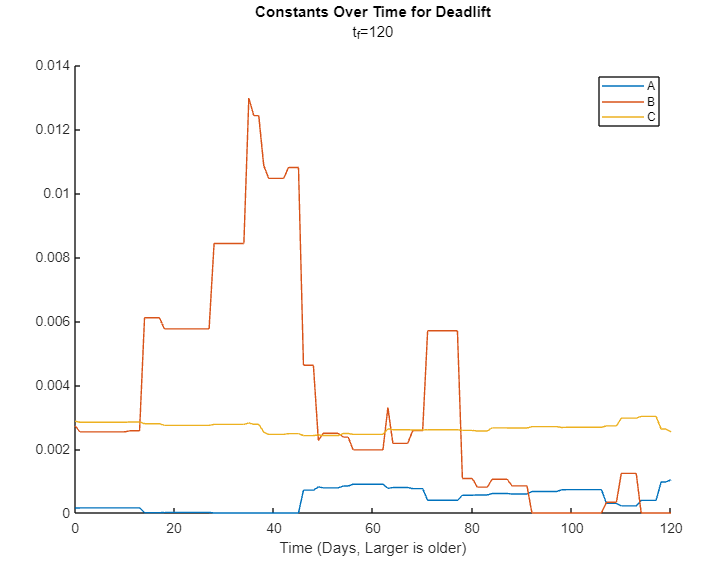
\includegraphics[width=140mm]{DeadliftConstants/abc.png}
%    \caption{The value of constants over time for deadlift when using a time frame of $120$ days. As the graph moves to the right the values are older.}
%    \label{fig:DeadliftConstantsOverTime}
%\end{figure}
%\begin{figure}[h]
%    \centering
%    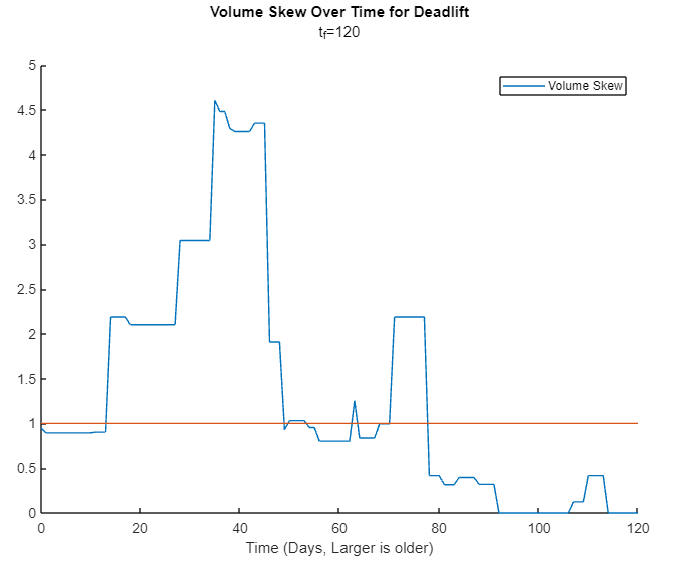
\includegraphics[width=140mm]{DeadliftConstants/VolumeSkew.png}
%    \caption{Volume skew over time for deadlift when using a time frame of $120$ days. As the graph moves to the right the values are older.}
%    \label{fig:DeadliftVolumeSkewOverTime}
%\end{figure}

\section{Analysis: Unbounded Volume}
\label{sec:PotentialSurfaceUnboundedVolume}

Unbounded volume occurs when volume continually increases. Unbounded volume is obviously not possible for a lifter to complete, and is especially problematic considering the purpose of this entire section is to establish what is possible and what is not possible. The boundary between bounded and unbounded volume needs to be found so that when this model is used in practice it works as anticipated.

If volume can be shown to have a global maximum, it can be stated that volume is bounded, or does not increase indefinitely. To prove volume has a peak requires the first partial and second partial derivative of $v$. The partial derivative with respect to $s$ was chosen. It will be discussed later what changes when the partial derivative with respect to $r$ is chosen instead.

\begin{equation}
    \label{eq:IntensitySubedInVolume}
    v(s,r,E)=sr\left( d-a(s-1)^2(r-1)^2-b(s-1)^2-c(r-1)^2-\epsilon E \right)
\end{equation}
\begin{equation}
    \label{eq:VolumeSPartialDerivative}
    \frac{\partial v}{\partial s}=rd-r\epsilon E-cr(r-1)^2-r\left( a(r-1)^2+b \right)\left( 3s^2-4s+1 \right)
\end{equation}
\begin{equation}
    \label{eq:VolumeSSecondPartialDerivative}
    \frac{\partial v'}{\partial s}=-(r)\left( a(r-1)^2+b \right)(6s-4)
\end{equation}

A global maximum occurs when $\partial_{ss} v<0$. In order for this to be the case an even number of the above parenthetical groupings need to be negative. The first parenthetical grouping is always guaranteed to be greater than $1$ from the constraints placed on $r$ in section \ref{sec:UnitsOfMeasurement}. The last parenthetical grouping will be $>0$ if $s>\frac{2}{3}$, which is again guaranteed to be true because of the constraints placed on $s$ in section \ref{sec:UnitsOfMeasurement}. This guarantees two of the three parenthetical groupings to be positive, which forces the middle parenthetical grouping to be positive for $\partial_{ss} v$ to be $<0$. The sign of $a$ changes the set of inequalities that define when the middle parenthetical group is $>0$, and hence when a maximum can occur. Table \ref{tab:BoundedVolumeRanges} shows the inequalities and ranges when volume is bounded for various values of $a$ and $b$.

Care has to be taken when $a=0$ or $b=0$, as the behavior of the inequalities is not fully captured by substituting $0$ for $a$ or $b$. A traditional limit cannot be used because inequalities are one sided, and a limit expects a continuous function. Instead, the four scenarios where $a=0$ and $b=0$ will be treated as one sided limits which will be approached from the side where the behavior is already known. By doing this, the sign can be inferred and the one sided nature of the problem can be handled. \footnote{The notation used in table \ref{tab:BoundedVolumeRanges} is as follows: given a number $x$, $x^-$ is a smaller number approaching $x$, and $x^+$ is a larger number approaching $x$. This allows for one sided analysis to be completed.} The scenarios where the root is imaginary are also troublesome. However, the same one sided analysis can be extended and used again. Looking at table \ref{tab:BoundedVolumeRanges} it should be clear how the one sided limit works as well as how the ranges over which volume is bounded respond.

\begin{table}[h]
    \centering
    \begin{tabular}{c|p{6cm}|c}
        Values for $a$ and $b$ & Inequalities & Range Where Volume is Bounded \\
        \hline

        $a>0$ and $b<0$
        &
        $r> \left(-\frac{b}{a}\right)^\frac{1}{2}+1$
        \newline
        $r< -\left(-\frac{b}{a}\right)^\frac{1}{2}+1$
        &
        $\left( r>\left| \frac{b}{a} \right|^\frac{1}{2}+1 \right) \cup \left( r< -\left| \frac{b}{a} \right|^\frac{1}{2}+1 \right)$
        \\
        \hline
        
        $a>0$ and $b=0$
        &
        $r> \left(-\frac{0^-}{a}\right)^\frac{1}{2}+1$
        \newline
        $r< -\left(-\frac{0^-}{a}\right)^\frac{1}{2}+1$
        &
        $\left( r> 1^+ \right) \cup \left( r<1^- \right)$, a.k.a. $r\ne 1$
        \\
        \hline
        
        $a>0$ and $b>0$
        &
        $r> (0+\beta i)+1$
        \newline
        $r< (-0-\beta i)+1$
        &
        $(r>1)\cup (r<1)$ a.k.a. All $r$
        \\
        \hline
        
        $a=0$ and $b>0$
        &
        $r> \left(-\frac{b}{0^+}\right)^\frac{1}{2}+1=(0+\infty i)+1$
        \newline
        $r< -\left(-\frac{b}{0^+}\right)^\frac{1}{2}+1=(-0-\infty i)+1$
        &
        $(r>1)\cup (r<1)$ a.k.a. All $r$
        \\
        \hline
        
        $a<0$ and $b>0$
        &
        $r< \left(-\frac{b}{a}\right)^\frac{1}{2}+1$
        \newline
        $r> -\left(-\frac{b}{a}\right)^\frac{1}{2}+1$
        &
        $-\left| \frac{b}{a} \right|^\frac{1}{2}+1 < r< \left| \frac{b}{a} \right|^\frac{1}{2}+1$
        \\
        \hline
        
        $a<0$ and $b=0$
        &
        $r< \left(-\frac{0^+}{a}\right)^\frac{1}{2}+1$
        \newline
        $r> -\left(-\frac{0^+}{a}\right)^\frac{1}{2}+1$
        &
        $1^- < r< 1^+$, a.k.a. Never
        \\
        \hline
        
        $a<0$ and $b<0$
        &
        $r< (0+\beta i)+1$
        \newline
        $r> (-0-\beta i)+1$
        &
        $1<r<1$ a.k.a. Never
        \\
        \hline
        
        $a=0$ and $b<0$
        &
        $r< \left(-\frac{b}{0^-}\right)^\frac{1}{2}+1=(0+\infty i)+1$
        \newline
        $r> -\left(-\frac{b}{0^-}\right)^\frac{1}{2}+1=(-0-\infty i)+1$
        &
        $1<r<1$ a.k.a. Never
        \\
    \end{tabular}
    \caption{Various values for $a$ and $b$ as well as there resulting ranges where volume is bounded.}
    \label{tab:BoundedVolumeRanges}
\end{table}

Given the ranges where a maximum could occur, a critical point is still needs to be found, which will require setting $\partial_sv$ equal to $0$. After algebraic manipulation, equation \ref{eq:VolumeRidgeConstR} is generated.
%Using the quadratic formula and substituting $\alpha_s$ in place of the fraction for ease of writing, the following points are generated as critical points.

%the equation below is generated.
\begin{equation}
    \label{eq:VolumeRidgeConstR}
    3s^2-4s+\left( 1-\frac{d-c(r-1)^2-\epsilon E}{a(r-1)^2-b} \right)=0
\end{equation}

 Using the quadratic formula and substituting $\alpha_s$ in place of the fraction for ease of writing, the following points are generated as critical points.
 
\begin{equation*}
    s=\frac{2\pm \sqrt{1+3\alpha_s}}{3}
\end{equation*}

From here the determinant can be used to show where critical points well occur.

\begin{enumerate}
    \item $\alpha_s < -\frac{1}{3}$: No critical points
    \item $\alpha_s = -\frac{1}{3}$: Indeterminate critical point
    \item $\alpha_s > -\frac{1}{3}$: Two critical points
\end{enumerate}

Given the above scenarios for critical points, only option $(3)$ is of interest. As shown below, if $\alpha_s> -\frac{1}{3}$ one critical point is generated on either side of $s=\frac{2}{3}$, the exact $s$ boundary where $\partial_{ss} v$ changes sign. Again, $\partial_{ss} v$ needs to $<0$ for a maximum to be found, requiring the parenthetical relating to $s$ in $\partial_{ss} v$ to be $>0$. This further narrows down the critical points to only include the one that is $>\frac{2}{3}$. It is worth mentioning that this is also the only valid critical point from the context of the problem, with $s$ being constrained to be $>1$ in section \ref{sec:UnitsOfMeasurement}.

\begin{equation*}
    s=\frac{2\pm \sqrt{1+3\left( -\frac{1}{3} \right)^+}}{3}=\frac{2\pm 0^+}{3}=\left( \frac{2}{3} \right)^-, \left( \frac{2}{3} \right)^+
\end{equation*}

Given that $\alpha_s>-\frac{1}{3}$, there will be a critical point. This can now be combined with the ranges where volume is bounded as well as the context of the problem to create the following statements:

\begin{enumerate}
    \item Volume is fully bounded for all $r$ when $a,b>0$.
    \item When $a>0$ and $b=0$ volume is fully bounded for all $r\ne 1$.
    \item When $a<0$ and $b=0$ volume is never bounded.
    \item When $a=0$ and $b>0$, volume is fully bounded.
    \item When $a=0$ and $b<0$, volume is never bounded.
    \item When $a>0$ and $b<0$, volume is bounded for $r>\left| \frac{b}{a} \right|^\frac{1}{2}+1$.
    \item When $a<0$ and $b>0$, volume is bounded for $1\le r < \left| \frac{b}{a} \right|^\frac{1}{2}+1$
\end{enumerate}

This analysis only looked at sets, which was an assumption made from the very beginning when the partial derivative of $v$ was taken with respect to $s$. If instead, the partial derivative was taken with respect to $r$, an analogous process would be followed. Due to the symmetry from $\partial_sv$ and $\partial_rv$, the only differences will be $c$ replacing $b$, $\alpha_r$ replacing $\alpha_s$ and, obviously, $s$ and $r$ switching roles. This creates the following additional statements given that $\alpha_r>-\frac{1}{3}$:

\begin{enumerate}
    \setcounter{enumi}{7}
    \item Volume is fully bounded for all $s$ when $a,c>0$.
    \item When $a>0$ and $c=0$ volume is fully bounded for all $s\ne 1$.
    \item When $a<0$ and $c=0$ volume is never bounded.
    \item When $a=0$ and $c>0$, volume is fully bounded.
    \item When $a=0$ and $c<0$, volume is never bounded.
    \item When $a>0$ and $c<0$, volume is bounded for $s>\left| \frac{c}{a} \right|^\frac{1}{2}+1$.
    \item When $a<0$ and $c>0$, volume is bounded for $1\le s < \left| \frac{c}{a} \right|^\frac{1}{2}+1$
\end{enumerate}

For peace of mind, figure \ref{fig:VolumeConstSRPeak} shows the peak volume identified by the above algebraic analysis. There is a peak for all $s$ and $r$ values, which means that volume is fully bounded. This also matches the statements above as $a=1.6\times 10^{-4}$, $b=2.7\times 10^{-3}$, and $c=2.9\times 10^{-3}$, which are all greater than $0$.

\begin{figure}[h]
    \centering
    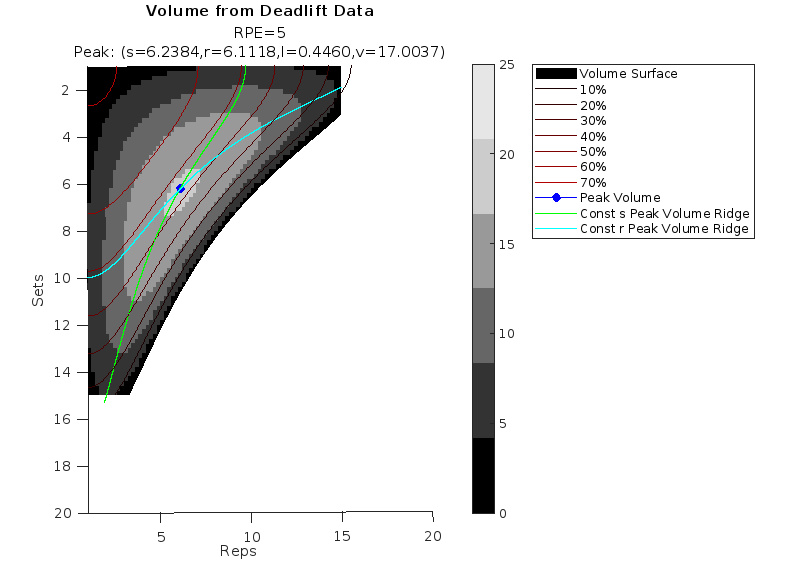
\includegraphics[width=170mm]{DeadliftVolume/FailedRidgeIdentification-2.png}
    \caption{The peak identified in volume given constant $s$ and $r$ values. This may look similar to figure \ref{fig:DeadliftIntensityCriticalPointsOnVolume} but they are two different graphs that were generated from two different approaches.}
    \label{fig:VolumeConstSRPeak}
\end{figure}

The above statements make sense in isolation, but when considered together things can contradict each other. If $a<0$, $b=0$, and $c>0$, then  statement $(3)$ states volume is never bounded, but statement $(14)$ states volume is bounded for a specific region. Again, this is the result of looking at a three dimensional problem from two dimensions, and is the same reason why the two peak volume lines in figure \ref{fig:VolumeConstSRPeak} do not coincide. While this does create some problems, the above statements are still is able to give some intuition for the problem at hand. Revisiting the example stated previously, it is saying that volume from reps is never bounded, and volume from sets is only bounded over a region. This intuition can be used to adjust training appropriately to avoid unbounded volume.

It is tempting to say the bounds in the above statements can be used in practice to limit the lifter from doing to much volume, but just because volume is bounded does not mean it is reasonable. Just because it can be proven that volume has a peak does not prove that the peak volume is attainable. This is a limitation of the model that stems from using linear regression to fit a surface to the data. Linear regression will implicitly extrapolate what amount of volume can be done given the data it has. Extrapolation is a known weakness of linear regression, making its predicted volume sometimes inaccurate.

To simplify the model, $b$ and $c$ can be limited to being $\ge 0$ so that volume will only ever be unbounded when $b=0$ or $c=0$. Not only does this remove the complexities of defining ranges over which the potential surface has bounded volume, but it makes intuitive sense to limit the model to only describing what is possible.

\section{Application: Solving for the Unknown}
\label{sec:PotentialSurfaceSolvingForTheUnknown}

With the model presented so far, one of the variables can be solved for given some combination of sets, reps, effort, or weight. This is useful because it can give a lifter information they otherwise would have guessed. Equations \ref{eq:PotentialSurfaceSetsEquation} through \ref{eq:PotentialSurfaceEffortEquation} are the potential surface solved for various variables.

\begin{subequations}
    \begin{align}
        s(r,I,E)&=
        \left( 
            \frac{
                d-I-c(r-1)^2-\epsilon E
            }{
                a(r-1)^2+b
            }
        \right)^\frac{1}{2}+1
        \label{eq:PotentialSurfaceSetsEquation}\\
        r(s,I,E)&=
        \left(
            \frac{
                d-I-b(s-1)^2-\epsilon E
            }{
                a(s-1)^2+c
            }
        \right)^\frac{1}{2}+1
        \label{eq:PotentialSurfaceRepsEquation}\\
        I(s,r,E)&=
        d-a(s-1)^2(r-1)^2-b(s-1)^2-c(r-1)^2-\epsilon E
        \label{eq:PotentialSurfaceIntensityEquation}\\
        E(s,r,I)&=
        \frac{
            d-I-a(s-1)^2(r-1)^2-b(s-1)^2-c(r-1)^2
        }{
            \epsilon
        }
        \label{eq:PotentialSurfaceEffortEquation}
    \end{align}
\end{subequations}

As an example of using the above equations, a lifter is often concerned with estimating an updated 1RM for an exercise after completing some training. Increases in weight for a lifts 1RM is a sign of progress and successful training. The model presented already estimates a users current 1RM, just in a round-about way. A 1RM will be a maximal effort lift with one set of one rep. Given these parameters, the weight lifted can be found using equation \ref{eq:PotentialSurfaceIntensityEquation}, which can just be multiplied by the weight of the lifters known 1RM to get the weight of the lifters predicted 1RM, as shown in equation \ref{eq:1RMPrediction}.

\begin{equation}
    \label{eq:1RMPrediction}
    n_{1RM}=I(s=1,r=1,E=10)l_{1RM}=l_{1RM}( d-10\epsilon )
\end{equation}

It is worth taking a step back to understand what equation \ref{eq:1RMPrediction} is saying. The new 1RM is generated from a baseline value, $d$, which increases with effort, $10\epsilon$. \footnote{Remember, $\epsilon$ needs to be $<0$ for the model to behave appropriately. This was discussed in section \ref{sec:PotentialSurfaceVolumeIncreasesWithEffort}.} This intuitively makes sense, as the more effort a lifter exerts the greater there 1RM is should be.

To test the accuracy of equation \ref{eq:1RMPrediction}, the model can be made to fit to data before a 1RM attempt and then compare the predicted 1RM to the actual 1RM. The lifter had two competitions where 1RM's were tested: the first was deadlift only and the second was a full meet. The predicted and actual 1RM's for all the exercises performed at each competition are summarized in table \ref{tab:1RMPredictedVsActual}.

\begin{table}[h]
    \centering
    \begin{tabular}{p{2cm}|p{2cm}|p{2cm}|p{2cm}|p{2cm}|p{2cm}|p{2cm}}
        Exercise & Date & Time Frame (Days) & Current Time (Days) & Predicted 1RM (lbs) & Actual 1RM (lbs) & Difference (lbs) \\
        \hline
        
        Deadlift & 5/5/2022 & $40$ & $81$ & $506$ & $520$ & $14$ \\
        Squat & 7/24/2022 & $120$ & $1$ & $415$ & $435$ & $20$ \\
        Bench & 7/24/2022 & $120$ & $1$ & $267$ & $270$ & $3$ \\
        Deadlift & 7/24/2022 & $120$ & $1$ & $511$ & $535$ & $24$ \\
    \end{tabular}
    \caption{Predicted vs actual 1RM's. All weight values are rounded to the nearest pound.}
    \label{tab:1RMPredictedVsActual}
\end{table}

The model consistently under-predicts the lifters 1RM, and the largest difference in the predicted vs actual 1RM is $24$ lbs. The smallest difference is $3$ lbs. The time frames were chosen to limit the data to only data points after $3/27/2022$, which is the date of the first successful workout after the lifter sustained an injury and took two weeks off from the gym entirely. Section \ref{sec:PotetentialSurfaceImprovingAccuracy} will work towards improving the accuracy of the predicted 1RM.

%As with section \ref{sec:PotentialSurfaceAbstractlyDescribingTraining}, a lifters 1RM can be tracked across time, providing another way to describe training over time. Figure \ref{fig:Deadlift1RMOverTime} shows the models predicted 1RM over time. Again, while presented here as an application of the model, more will be gained from figure \ref{fig:Deadlift1RMOverTime} in section \ref{sec:Macrocycle}.
%
%\begin{figure}[h]
%    \centering
%    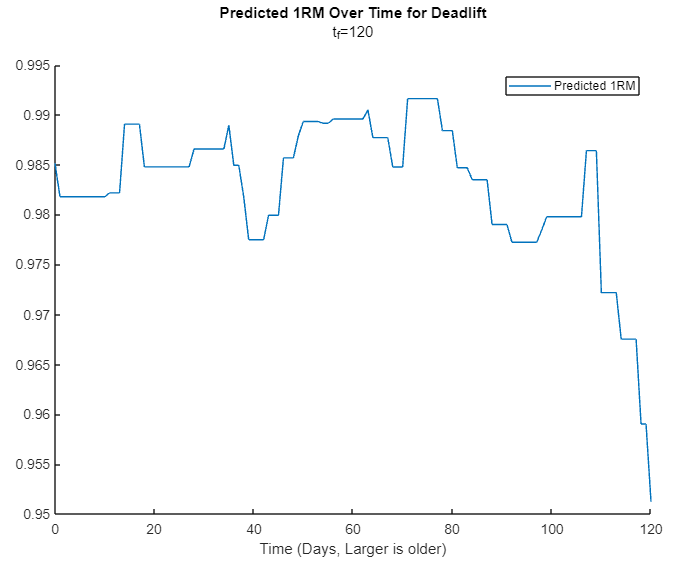
\includegraphics[width=140mm]{DeadliftConstants/pred1RM.png}
%    \caption{The models predicted 1RM over time for deadlift.}
%    \label{fig:Deadlift1RMOverTime}
%\end{figure}

\section{Improving Accuracy: Improvising for What's Not Included}
\label{sec:PotetentialSurfaceImprovingAccuracy}

Fatigue was presented in section \ref{sec:CommonTermsSection}, but until this point was not considered. This is mainly because it is not part of the data set that was used to generate the potential surface. Fatigue directly limits what can be lifted. This makes intuitive sense: a lifter that is fatigued will be tired and hence will not able to lift as much weight. This is one of the reasons why it gets harder to lift a given weight the more times it is attempted. Given this, if fatigue were to be added to the model it may look like something like equation \ref{eq:PotentialSurfaceEquationWithFatigue}, where $F$ is used to represent fatigue.

\begin{equation}
    \label{eq:PotentialSurfaceEquationWithFatigue}
    a(s-1)^2(r-1)^2+b(s-1)^2+c(r-1)^2+\epsilon E+\epsilon_2 F=d-I
\end{equation}

While fatigue cannot be represented directly by the model due to it not being part of the data, its affects should still be sought to be minimized. Within the broad category of fatigue, there two sub-types: \textit{inter-workout} and \textit{inter-exercise} fatigue. As the names suggest, inter-workout fatigue is fatigue that accumulates over the course of an entire workout, and inter-exercise fatigue is fatigue that accumulates over the course of a single exercise. When a lifter switches exercises fatigue drops depending on the amount of similarity between the exercises. If two exercises are similar more fatigue will carry over between them, increasing both the perceived inter-workout fatigue as well as the inter-exercise fatigue on the second exercise. On some occasions this is purposeful, and is used as a way to increase stimulus while keeping intensity low.

It should be obvious that effects from inter-workout fatigue cannot be minimized, as this surface is only defined for a single exercise, but the effects from inter-exercise fatigue can be partially controlled for. If the same exercise is performed on the same day with different weights, then each set with a different weight can be given an 'index' to show the order that the sets occurred in.\footnote{This obviously only includes working sets. Warm up sets will not be indexed.} This order will then take the place of a fatigue measurement, and linear regression can be completed using the augmented data set. While not perfect, this works because the index increases as fatigue would increase, creating a way to test if having actual fatigue data would increase the accuracy of the model. This 'index' will be called the \textit{fatigue index} and will will start at $0$ to reflect that the first set done will have no fatigue. If the value for $\epsilon_2$ from linear regression is not near $0$ then it can be said fatigue significantly contributes to the model. Table \ref{tab:LinearRegressionConstantsWithFatigue} shows the results after completing linear regression on deadlift data with the new augmented data set. It is clear, when compared to the other constants, the $\epsilon_2$ constant is large enough to be significant.

\begin{table}[h]
    \centering
    \begin{tabular}{c|c|c|c|c|c|c}
         & $a$ & $b$ & $c$ & $d$ & $\epsilon$ & $\epsilon_2$ \\
         \hline
        With Fatigue Index & $0.0001$ & $0.0029$ & $0.0028$ & $0.4179$ & $-0.0519$ & $0.0173$ \\
        Without Fatigue Index & $0.0002$ & $0.0027$ & $0.0029$ & $0.4302$ & $-0.0555$ & - \\
    \end{tabular}
    \caption{Linear regression constants from deadlift data with and without the augmented fatigue data.}
    \label{tab:LinearRegressionConstantsWithFatigue}
\end{table}

Despite augmenting the data set and adding a new variable, much of the work outlined in sections \ref{sec:PotentialSurfaceVolumeIncreasesWithEffort}-\ref{sec:PotentialSurfaceSolvingForTheUnknown} remains unaffected, as the added fatigue term either drops out after performing differentiation or just tags along similar to the effort term. The changes to equations \ref{eq:PotentialSurfaceSetsEquation}-\ref{eq:PotentialSurfaceEffortEquation} are shown in equations \ref{eq:PotentialSurfaceSetsEquationWithFatigue}-\ref{eq:PotentialSurfaceEffortEquationWithFatigue} for convenience.

\begin{subequations}
    \begin{align}
        s(r,I,E,F)&=
        \left( 
            \frac{
                d-I-c(r-1)^2-\epsilon E-\epsilon_2 F
            }{
                a(r-1)^2+b
            }
        \right)^\frac{1}{2}+1
        \label{eq:PotentialSurfaceSetsEquationWithFatigue}\\
        r(s,I,E,F)&=
        \left(
            \frac{
                d-I-b(s-1)^2-\epsilon E-\epsilon_2 F
            }{
                a(s-1)^2+c
            }
        \right)^\frac{1}{2}+1
        \label{eq:PotentialSurfaceRepsEquationWithFatigue}\\
        I(s,r,E,F)&=
        d-a(s-1)^2(r-1)^2-b(s-1)^2-c(r-1)^2-\epsilon E-\epsilon_2 F
        \label{eq:PotentialSurfaceIntensityEquationWithFatigue}\\
        E(s,r,I,F)&=
        \frac{
            d-I-a(s-1)^2(r-1)^2-b(s-1)^2-c(r-1)^2-\epsilon_2 F
        }{
            \epsilon
        }
        \label{eq:PotentialSurfaceEffortEquationWithFatigue}\\
        F(s,r,I,E)&=
        \frac{
            d-I-a(s-1)^2(r-1)^2-b(s-1)^2-c(r-1)^2 -\epsilon E
        }{
            \epsilon_2
        }
        \label{eq:PotentialSurfaceFatigueEquation}
    \end{align}
\end{subequations}

%As equation \ref{eq:PotentialSurfaceFatigueEquation} demonstrates, the fatigue index value can also be solved for, which presents an interesting opportunity to measure how fatigued a lifter is based on there previous lifts. Through equation \ref{eq:PotentialSurfaceEffortEquationWithFatigue}, the model will be able to predict a fatigue index. This fatigue index can then be compared to the actual fatigue index, and the delta can be used to show how fatigued you are compared to what the model expects. Equation \ref{eq:}

The changes to equation \ref{eq:1RMPrediction}, as shown in equation \ref{eq:1RMPredictionWithFatigue}, are also important. With the new predicted 1RM equation, there is still a baseline value, $d$, which increases with effort, $10\epsilon$, but the baseline value now decreases with fatigue, $\epsilon_2 F$. Again, this intuitively makes sense. If a lifter is in a fatigued state, they will not be able to lift as much weight, even with high amounts of effort. Put another way: performance is effort minus fatigue.
 
\begin{equation}
    \label{eq:1RMPredictionWithFatigue}
    n_{1RM}=I(s=1,r=1,E=10,F)l_{1RM}=l_{1RM}( d-10\epsilon-\epsilon_2 F)
\end{equation}

The updated 1RM prediction equation can be compared to the old one to see which one is more accurate. Table \ref{tab:Predicted1RMWithAndWithoutFatigue} compares the estimated 1RM's between the augmented data set and the non-augmented data set. The same lifts and time frames are used as table \ref{tab:1RMPredictedVsActual}. When computing the predicted 1RM with fatigue, a fatigue index of $F=0$ was used, as a 1RM attempt is usually the first set performed to avoid any affects from fatigue.

\begin{table}[h]
    \centering
    \begin{tabular}{p{2cm}|p{2cm}|p{3cm}|p{3cm}|p{3cm}}
        Exercise &  Date & Pred. 1RM With $F$  (lbs) & Pred. 1RM Without $F$ (lbs) & Actual 1RM (lbs) \\
        \hline
        Deadlift & 5/5/2022 & $506$ & $506$ & $520$ \\
        Squat & 7/24/2022 & $417$ & $415$ & $435$ \\
        Bench & 7/24/2022 & $269$ & $267$ & $270$ \\
        Deadlift & 7/24/2022 & $514$ & $511$ & $535$ \\
    \end{tabular}
    \caption{Predicted 1RM with and without the augmented fatigue data.}
    \label{tab:Predicted1RMWithAndWithoutFatigue}
\end{table}

As shown in table \ref{tab:Predicted1RMWithAndWithoutFatigue}, when the model is augmented with the fatigue index it has either the same or greater accuracy when predicting a 1RM, especially on bench, with the model being within $1$ pound of the users actual 1RM.

The affects of $\epsilon_2$ on $I$ also need to be considered to ensure the model is appropriately responding to fatigue. As such, the changes in $I$ relating to changes in $F$ are desired, requiring the derivative of equation \ref{eq:PotentialSurfaceEffortEquationWithFatigue} with respect to $F$. 

\begin{equation}
    \label{eq:VolumeFPartialDerivative}
    \frac{\partial I}{\partial F}=\frac{\partial}{\partial F} d-a(s-1)^2(r-1)^2-b(s-1)^2-c(r-1)^2-\epsilon E-\epsilon_2 F=-\epsilon_2
\end{equation}

As stated at the start of this section, fatigue limits what can be lifted. As such, $I$ needs to decrease as $\epsilon_2$ increases, requiring $\partial_F I<0$. It should be obvious that this can only happen if $\epsilon_2>0$, meaning that intensity decreases with fatigue \textbf{iff} $\epsilon_2>0$. Given the values for $\epsilon_2$ in table \ref{tab:Epsilon2AcrossExercises}, which are all positive, it is clear the model is appropriately identifying patterns in fatigue.

\begin{table}[h]
    \centering
    \begin{tabular}{c|c}
        Exercise & $\epsilon_2$ \\
        \hline
        Squat & $0.0116$ \\
        Bench & $0.0301$ \\
        Deadlift & $0.0173$ \\
    \end{tabular}
    \caption{The $\epsilon_2$ values for three different exercises. They are all positive, meaning the model is correctly making intensity decrease with increased fatigue.}
    \label{tab:Epsilon2AcrossExercises}
\end{table}

Augmenting the data with the fatigue index clearly improved the accuracy of the model, it is still not perfect. While the fatigue index does have the same general behavior as fatigue, it is not the exact same behavior. One difference is that fatigue will accumulate across all sets, not just across sets with a different weight. If each set was given an increasing fatigue index, regardless of weight, the model would no longer be able to accurately understand sets because every exercise would be split up into a list of single sets with a certain number of reps and an incrementing fatigue index. Splitting the data points apart like this would also create dependencies between the data points, which cannot happen with linear regression. To make sure the model accurately understands the relation between sets and reps, the fatigue index was made to only increase across sets of different weight. This has the unfortunate side effect of giving the fatigue index behavior that fatigue does not have, but is necessary to keep the rest of the model consistent.

All this consideration with the fatigue index raises the question: why not just create a new data set that records fatigue? Arguably, using actual fatigue data would give better results. The problem is that fatigue is hard to measure. A simple system like RPE cannot be used because often times a lifter may by psychologically fatigued, but physically they are fine, or visa versa. As John Broz, an Olympic trainer, says, "How you feel is a lie." While John has an extreme take on the discrepancy between how a lifter feels and how they perform, there is still some level of truth to the statement. There are many cases where a lifters psychological state does not match there physical state, resulting in discrepancies between what they think they can do and what they actually do during a workout. As such, simply asking a lifter to record how fatigued they feel on a given day is not going to produce reliable data. Other methods of measuring fatigue exist\cite{MEASURING_FATIGUE}, but these methods are generally not conducive to a training environment, which is where they would need to be used to capture changes in fatigue across sets. Finding a way to reliably record fatigue data while training will remain an unanswered question.

Due to the increased accuracy of the model with the fatigue index added to the data set, the rest of the paper will continue to use this updated model, which will be called the \textit{fatigue aware potential surface}.

%This is promising, and all seems well until volume skew is considered. Looking at $b$ and $c$ in table \ref{tab:LinearRegressionConstantsWithFatigue}, it should be obvious that the volume skew shifted. The volume skew without $F$ is $0.9495$, but with $F$ it is $1.0361$. Remembering the definition of volume skew, this means volume went from favoring sets to favoring reps. Looking at the graph from the raw data in figure \ref{fig:SetsVsReps} it should be clear the the model should favor sets, not reps.

%\section{Time Frame Considerations}
%\label{sec:PotentialSurfaceTimeFrameConsiderations}

